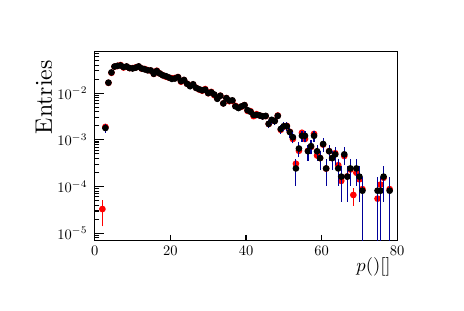
\begin{tikzpicture}
\pgfdeclareplotmark{cross} {
\pgfpathmoveto{\pgfpoint{-0.3\pgfplotmarksize}{\pgfplotmarksize}}
\pgfpathlineto{\pgfpoint{+0.3\pgfplotmarksize}{\pgfplotmarksize}}
\pgfpathlineto{\pgfpoint{+0.3\pgfplotmarksize}{0.3\pgfplotmarksize}}
\pgfpathlineto{\pgfpoint{+1\pgfplotmarksize}{0.3\pgfplotmarksize}}
\pgfpathlineto{\pgfpoint{+1\pgfplotmarksize}{-0.3\pgfplotmarksize}}
\pgfpathlineto{\pgfpoint{+0.3\pgfplotmarksize}{-0.3\pgfplotmarksize}}
\pgfpathlineto{\pgfpoint{+0.3\pgfplotmarksize}{-1.\pgfplotmarksize}}
\pgfpathlineto{\pgfpoint{-0.3\pgfplotmarksize}{-1.\pgfplotmarksize}}
\pgfpathlineto{\pgfpoint{-0.3\pgfplotmarksize}{-0.3\pgfplotmarksize}}
\pgfpathlineto{\pgfpoint{-1.\pgfplotmarksize}{-0.3\pgfplotmarksize}}
\pgfpathlineto{\pgfpoint{-1.\pgfplotmarksize}{0.3\pgfplotmarksize}}
\pgfpathlineto{\pgfpoint{-0.3\pgfplotmarksize}{0.3\pgfplotmarksize}}
\pgfpathclose
\pgfusepathqstroke
}
\pgfdeclareplotmark{cross*} {
\pgfpathmoveto{\pgfpoint{-0.3\pgfplotmarksize}{\pgfplotmarksize}}
\pgfpathlineto{\pgfpoint{+0.3\pgfplotmarksize}{\pgfplotmarksize}}
\pgfpathlineto{\pgfpoint{+0.3\pgfplotmarksize}{0.3\pgfplotmarksize}}
\pgfpathlineto{\pgfpoint{+1\pgfplotmarksize}{0.3\pgfplotmarksize}}
\pgfpathlineto{\pgfpoint{+1\pgfplotmarksize}{-0.3\pgfplotmarksize}}
\pgfpathlineto{\pgfpoint{+0.3\pgfplotmarksize}{-0.3\pgfplotmarksize}}
\pgfpathlineto{\pgfpoint{+0.3\pgfplotmarksize}{-1.\pgfplotmarksize}}
\pgfpathlineto{\pgfpoint{-0.3\pgfplotmarksize}{-1.\pgfplotmarksize}}
\pgfpathlineto{\pgfpoint{-0.3\pgfplotmarksize}{-0.3\pgfplotmarksize}}
\pgfpathlineto{\pgfpoint{-1.\pgfplotmarksize}{-0.3\pgfplotmarksize}}
\pgfpathlineto{\pgfpoint{-1.\pgfplotmarksize}{0.3\pgfplotmarksize}}
\pgfpathlineto{\pgfpoint{-0.3\pgfplotmarksize}{0.3\pgfplotmarksize}}
\pgfpathclose
\pgfusepathqfillstroke
}
\pgfdeclareplotmark{newstar} {
\pgfpathmoveto{\pgfqpoint{0pt}{\pgfplotmarksize}}
\pgfpathlineto{\pgfqpointpolar{44}{0.5\pgfplotmarksize}}
\pgfpathlineto{\pgfqpointpolar{18}{\pgfplotmarksize}}
\pgfpathlineto{\pgfqpointpolar{-20}{0.5\pgfplotmarksize}}
\pgfpathlineto{\pgfqpointpolar{-54}{\pgfplotmarksize}}
\pgfpathlineto{\pgfqpointpolar{-90}{0.5\pgfplotmarksize}}
\pgfpathlineto{\pgfqpointpolar{234}{\pgfplotmarksize}}
\pgfpathlineto{\pgfqpointpolar{198}{0.5\pgfplotmarksize}}
\pgfpathlineto{\pgfqpointpolar{162}{\pgfplotmarksize}}
\pgfpathlineto{\pgfqpointpolar{134}{0.5\pgfplotmarksize}}
\pgfpathclose
\pgfusepathqstroke
}
\pgfdeclareplotmark{newstar*} {
\pgfpathmoveto{\pgfqpoint{0pt}{\pgfplotmarksize}}
\pgfpathlineto{\pgfqpointpolar{44}{0.5\pgfplotmarksize}}
\pgfpathlineto{\pgfqpointpolar{18}{\pgfplotmarksize}}
\pgfpathlineto{\pgfqpointpolar{-20}{0.5\pgfplotmarksize}}
\pgfpathlineto{\pgfqpointpolar{-54}{\pgfplotmarksize}}
\pgfpathlineto{\pgfqpointpolar{-90}{0.5\pgfplotmarksize}}
\pgfpathlineto{\pgfqpointpolar{234}{\pgfplotmarksize}}
\pgfpathlineto{\pgfqpointpolar{198}{0.5\pgfplotmarksize}}
\pgfpathlineto{\pgfqpointpolar{162}{\pgfplotmarksize}}
\pgfpathlineto{\pgfqpointpolar{134}{0.5\pgfplotmarksize}}
\pgfpathclose
\pgfusepathqfillstroke
}
\definecolor{c}{rgb}{1,1,1};
\draw [color=c, fill=c] (0.1,0.0624161) rectangle (4.9,3.05839);
\draw [color=c, fill=c] (0.58,0.362013) rectangle (4.42,2.75879);
\definecolor{c}{rgb}{0,0,0};
\draw [c] (0.58,0.362013) -- (0.58,2.75879) -- (4.42,2.75879) -- (4.42,0.362013) -- (0.58,0.362013);
\definecolor{c}{rgb}{1,0,0};
\draw [c] (0.676,0.540502) -- (0.676,0.762267);
\draw [c] (0.676,0.762267) -- (0.676,0.879624);
\draw [c] (0.6568,0.762267) -- (0.676,0.762267);
\draw [c] (0.676,0.762267) -- (0.6952,0.762267);
\foreach \P in {(0.676,0.762267)}{\draw[mark options={color=c,fill=c},mark size=2.402402pt,mark=*,mark size=1pt] plot coordinates {\P};}
\draw [c] (0.7144,1.78445) -- (0.7144,1.80487);
\draw [c] (0.7144,1.80487) -- (0.7144,1.82379);
\draw [c] (0.6952,1.80487) -- (0.7144,1.80487);
\draw [c] (0.7144,1.80487) -- (0.7336,1.80487);
\foreach \P in {(0.7144,1.80487)}{\draw[mark options={color=c,fill=c},mark size=2.402402pt,mark=*,mark size=1pt] plot coordinates {\P};}
\draw [c] (0.7528,2.35841) -- (0.7528,2.36512);
\draw [c] (0.7528,2.36512) -- (0.7528,2.37165);
\draw [c] (0.7336,2.36512) -- (0.7528,2.36512);
\draw [c] (0.7528,2.36512) -- (0.772,2.36512);
\foreach \P in {(0.7528,2.36512)}{\draw[mark options={color=c,fill=c},mark size=2.402402pt,mark=*,mark size=1pt] plot coordinates {\P};}
\draw [c] (0.7912,2.48712) -- (0.7912,2.49234);
\draw [c] (0.7912,2.49234) -- (0.7912,2.49745);
\draw [c] (0.772,2.49234) -- (0.7912,2.49234);
\draw [c] (0.7912,2.49234) -- (0.8104,2.49234);
\foreach \P in {(0.7912,2.49234)}{\draw[mark options={color=c,fill=c},mark size=2.402402pt,mark=*,mark size=1pt] plot coordinates {\P};}
\draw [c] (0.8296,2.5659) -- (0.8296,2.57038);
\draw [c] (0.8296,2.57038) -- (0.8296,2.57478);
\draw [c] (0.8104,2.57038) -- (0.8296,2.57038);
\draw [c] (0.8296,2.57038) -- (0.8488,2.57038);
\foreach \P in {(0.8296,2.57038)}{\draw[mark options={color=c,fill=c},mark size=2.402402pt,mark=*,mark size=1pt] plot coordinates {\P};}
\draw [c] (0.868,2.57501) -- (0.868,2.57941);
\draw [c] (0.868,2.57941) -- (0.868,2.58374);
\draw [c] (0.8488,2.57941) -- (0.868,2.57941);
\draw [c] (0.868,2.57941) -- (0.8872,2.57941);
\foreach \P in {(0.868,2.57941)}{\draw[mark options={color=c,fill=c},mark size=2.402402pt,mark=*,mark size=1pt] plot coordinates {\P};}
\draw [c] (0.9064,2.58568) -- (0.9064,2.58999);
\draw [c] (0.9064,2.58999) -- (0.9064,2.59423);
\draw [c] (0.8872,2.58999) -- (0.9064,2.58999);
\draw [c] (0.9064,2.58999) -- (0.9256,2.58999);
\foreach \P in {(0.9064,2.58999)}{\draw[mark options={color=c,fill=c},mark size=2.402402pt,mark=*,mark size=1pt] plot coordinates {\P};}
\draw [c] (0.9448,2.55493) -- (0.9448,2.55951);
\draw [c] (0.9448,2.55951) -- (0.9448,2.564);
\draw [c] (0.9256,2.55951) -- (0.9448,2.55951);
\draw [c] (0.9448,2.55951) -- (0.964,2.55951);
\foreach \P in {(0.9448,2.55951)}{\draw[mark options={color=c,fill=c},mark size=2.402402pt,mark=*,mark size=1pt] plot coordinates {\P};}
\draw [c] (0.9832,2.56644) -- (0.9832,2.57091);
\draw [c] (0.9832,2.57091) -- (0.9832,2.57531);
\draw [c] (0.964,2.57091) -- (0.9832,2.57091);
\draw [c] (0.9832,2.57091) -- (1.0024,2.57091);
\foreach \P in {(0.9832,2.57091)}{\draw[mark options={color=c,fill=c},mark size=2.402402pt,mark=*,mark size=1pt] plot coordinates {\P};}
\draw [c] (1.0216,2.54707) -- (1.0216,2.55172);
\draw [c] (1.0216,2.55172) -- (1.0216,2.55628);
\draw [c] (1.0024,2.55172) -- (1.0216,2.55172);
\draw [c] (1.0216,2.55172) -- (1.0408,2.55172);
\foreach \P in {(1.0216,2.55172)}{\draw[mark options={color=c,fill=c},mark size=2.402402pt,mark=*,mark size=1pt] plot coordinates {\P};}
\draw [c] (1.06,2.54732) -- (1.06,2.55197);
\draw [c] (1.06,2.55197) -- (1.06,2.55653);
\draw [c] (1.0408,2.55197) -- (1.06,2.55197);
\draw [c] (1.06,2.55197) -- (1.0792,2.55197);
\foreach \P in {(1.06,2.55197)}{\draw[mark options={color=c,fill=c},mark size=2.402402pt,mark=*,mark size=1pt] plot coordinates {\P};}
\draw [c] (1.0984,2.55517) -- (1.0984,2.55975);
\draw [c] (1.0984,2.55975) -- (1.0984,2.56424);
\draw [c] (1.0792,2.55975) -- (1.0984,2.55975);
\draw [c] (1.0984,2.55975) -- (1.1176,2.55975);
\foreach \P in {(1.0984,2.55975)}{\draw[mark options={color=c,fill=c},mark size=2.402402pt,mark=*,mark size=1pt] plot coordinates {\P};}
\draw [c] (1.1368,2.56705) -- (1.1368,2.57152);
\draw [c] (1.1368,2.57152) -- (1.1368,2.57592);
\draw [c] (1.1176,2.57152) -- (1.1368,2.57152);
\draw [c] (1.1368,2.57152) -- (1.156,2.57152);
\foreach \P in {(1.1368,2.57152)}{\draw[mark options={color=c,fill=c},mark size=2.402402pt,mark=*,mark size=1pt] plot coordinates {\P};}
\draw [c] (1.1752,2.54076) -- (1.1752,2.54547);
\draw [c] (1.1752,2.54547) -- (1.1752,2.55009);
\draw [c] (1.156,2.54547) -- (1.1752,2.54547);
\draw [c] (1.1752,2.54547) -- (1.1944,2.54547);
\foreach \P in {(1.1752,2.54547)}{\draw[mark options={color=c,fill=c},mark size=2.402402pt,mark=*,mark size=1pt] plot coordinates {\P};}
\draw [c] (1.2136,2.53569) -- (1.2136,2.54044);
\draw [c] (1.2136,2.54044) -- (1.2136,2.54511);
\draw [c] (1.1944,2.54044) -- (1.2136,2.54044);
\draw [c] (1.2136,2.54044) -- (1.2328,2.54044);
\foreach \P in {(1.2136,2.54044)}{\draw[mark options={color=c,fill=c},mark size=2.402402pt,mark=*,mark size=1pt] plot coordinates {\P};}
\draw [c] (1.252,2.52132) -- (1.252,2.5262);
\draw [c] (1.252,2.5262) -- (1.252,2.531);
\draw [c] (1.2328,2.5262) -- (1.252,2.5262);
\draw [c] (1.252,2.5262) -- (1.2712,2.5262);
\foreach \P in {(1.252,2.5262)}{\draw[mark options={color=c,fill=c},mark size=2.402402pt,mark=*,mark size=1pt] plot coordinates {\P};}
\draw [c] (1.2904,2.51538) -- (1.2904,2.52032);
\draw [c] (1.2904,2.52032) -- (1.2904,2.52517);
\draw [c] (1.2712,2.52032) -- (1.2904,2.52032);
\draw [c] (1.2904,2.52032) -- (1.3096,2.52032);
\foreach \P in {(1.2904,2.52032)}{\draw[mark options={color=c,fill=c},mark size=2.402402pt,mark=*,mark size=1pt] plot coordinates {\P};}
\draw [c] (1.3288,2.47368) -- (1.3288,2.47904);
\draw [c] (1.3288,2.47904) -- (1.3288,2.48428);
\draw [c] (1.3096,2.47904) -- (1.3288,2.47904);
\draw [c] (1.3288,2.47904) -- (1.348,2.47904);
\foreach \P in {(1.3288,2.47904)}{\draw[mark options={color=c,fill=c},mark size=2.402402pt,mark=*,mark size=1pt] plot coordinates {\P};}
\draw [c] (1.3672,2.51349) -- (1.3672,2.51845);
\draw [c] (1.3672,2.51845) -- (1.3672,2.52332);
\draw [c] (1.348,2.51845) -- (1.3672,2.51845);
\draw [c] (1.3672,2.51845) -- (1.3864,2.51845);
\foreach \P in {(1.3672,2.51845)}{\draw[mark options={color=c,fill=c},mark size=2.402402pt,mark=*,mark size=1pt] plot coordinates {\P};}
\draw [c] (1.4056,2.47784) -- (1.4056,2.48315);
\draw [c] (1.4056,2.48315) -- (1.4056,2.48836);
\draw [c] (1.3864,2.48315) -- (1.4056,2.48315);
\draw [c] (1.4056,2.48315) -- (1.4248,2.48315);
\foreach \P in {(1.4056,2.48315)}{\draw[mark options={color=c,fill=c},mark size=2.402402pt,mark=*,mark size=1pt] plot coordinates {\P};}
\draw [c] (1.444,2.45539) -- (1.444,2.46094);
\draw [c] (1.444,2.46094) -- (1.444,2.46638);
\draw [c] (1.4248,2.46094) -- (1.444,2.46094);
\draw [c] (1.444,2.46094) -- (1.4632,2.46094);
\foreach \P in {(1.444,2.46094)}{\draw[mark options={color=c,fill=c},mark size=2.402402pt,mark=*,mark size=1pt] plot coordinates {\P};}
\draw [c] (1.4824,2.43737) -- (1.4824,2.44312);
\draw [c] (1.4824,2.44312) -- (1.4824,2.44874);
\draw [c] (1.4632,2.44312) -- (1.4824,2.44312);
\draw [c] (1.4824,2.44312) -- (1.5016,2.44312);
\foreach \P in {(1.4824,2.44312)}{\draw[mark options={color=c,fill=c},mark size=2.402402pt,mark=*,mark size=1pt] plot coordinates {\P};}
\draw [c] (1.5208,2.42488) -- (1.5208,2.43077);
\draw [c] (1.5208,2.43077) -- (1.5208,2.43653);
\draw [c] (1.5016,2.43077) -- (1.5208,2.43077);
\draw [c] (1.5208,2.43077) -- (1.54,2.43077);
\foreach \P in {(1.5208,2.43077)}{\draw[mark options={color=c,fill=c},mark size=2.402402pt,mark=*,mark size=1pt] plot coordinates {\P};}
\draw [c] (1.5592,2.4169) -- (1.5592,2.42288);
\draw [c] (1.5592,2.42288) -- (1.5592,2.42873);
\draw [c] (1.54,2.42288) -- (1.5592,2.42288);
\draw [c] (1.5592,2.42288) -- (1.5784,2.42288);
\foreach \P in {(1.5592,2.42288)}{\draw[mark options={color=c,fill=c},mark size=2.402402pt,mark=*,mark size=1pt] plot coordinates {\P};}
\draw [c] (1.5976,2.41977) -- (1.5976,2.42572);
\draw [c] (1.5976,2.42572) -- (1.5976,2.43153);
\draw [c] (1.5784,2.42572) -- (1.5976,2.42572);
\draw [c] (1.5976,2.42572) -- (1.6168,2.42572);
\foreach \P in {(1.5976,2.42572)}{\draw[mark options={color=c,fill=c},mark size=2.402402pt,mark=*,mark size=1pt] plot coordinates {\P};}
\draw [c] (1.636,2.43211) -- (1.636,2.43792);
\draw [c] (1.636,2.43792) -- (1.636,2.4436);
\draw [c] (1.6168,2.43792) -- (1.636,2.43792);
\draw [c] (1.636,2.43792) -- (1.6552,2.43792);
\foreach \P in {(1.636,2.43792)}{\draw[mark options={color=c,fill=c},mark size=2.402402pt,mark=*,mark size=1pt] plot coordinates {\P};}
\draw [c] (1.6744,2.3733) -- (1.6744,2.37982);
\draw [c] (1.6744,2.37982) -- (1.6744,2.38617);
\draw [c] (1.6552,2.37982) -- (1.6744,2.37982);
\draw [c] (1.6744,2.37982) -- (1.6936,2.37982);
\foreach \P in {(1.6744,2.37982)}{\draw[mark options={color=c,fill=c},mark size=2.402402pt,mark=*,mark size=1pt] plot coordinates {\P};}
\draw [c] (1.7128,2.39332) -- (1.7128,2.39959);
\draw [c] (1.7128,2.39959) -- (1.7128,2.4057);
\draw [c] (1.6936,2.39959) -- (1.7128,2.39959);
\draw [c] (1.7128,2.39959) -- (1.732,2.39959);
\foreach \P in {(1.7128,2.39959)}{\draw[mark options={color=c,fill=c},mark size=2.402402pt,mark=*,mark size=1pt] plot coordinates {\P};}
\draw [c] (1.7512,2.34643) -- (1.7512,2.35329);
\draw [c] (1.7512,2.35329) -- (1.7512,2.35997);
\draw [c] (1.732,2.35329) -- (1.7512,2.35329);
\draw [c] (1.7512,2.35329) -- (1.7704,2.35329);
\foreach \P in {(1.7512,2.35329)}{\draw[mark options={color=c,fill=c},mark size=2.402402pt,mark=*,mark size=1pt] plot coordinates {\P};}
\draw [c] (1.7896,2.32126) -- (1.7896,2.32846);
\draw [c] (1.7896,2.32846) -- (1.7896,2.33547);
\draw [c] (1.7704,2.32846) -- (1.7896,2.32846);
\draw [c] (1.7896,2.32846) -- (1.8088,2.32846);
\foreach \P in {(1.7896,2.32846)}{\draw[mark options={color=c,fill=c},mark size=2.402402pt,mark=*,mark size=1pt] plot coordinates {\P};}
\draw [c] (1.828,2.33613) -- (1.828,2.34313);
\draw [c] (1.828,2.34313) -- (1.828,2.34994);
\draw [c] (1.8088,2.34313) -- (1.828,2.34313);
\draw [c] (1.828,2.34313) -- (1.8472,2.34313);
\foreach \P in {(1.828,2.34313)}{\draw[mark options={color=c,fill=c},mark size=2.402402pt,mark=*,mark size=1pt] plot coordinates {\P};}
\draw [c] (1.8664,2.29426) -- (1.8664,2.30185);
\draw [c] (1.8664,2.30185) -- (1.8664,2.30923);
\draw [c] (1.8472,2.30185) -- (1.8664,2.30185);
\draw [c] (1.8664,2.30185) -- (1.8856,2.30185);
\foreach \P in {(1.8664,2.30185)}{\draw[mark options={color=c,fill=c},mark size=2.402402pt,mark=*,mark size=1pt] plot coordinates {\P};}
\draw [c] (1.9048,2.27242) -- (1.9048,2.28034);
\draw [c] (1.9048,2.28034) -- (1.9048,2.28802);
\draw [c] (1.8856,2.28034) -- (1.9048,2.28034);
\draw [c] (1.9048,2.28034) -- (1.924,2.28034);
\foreach \P in {(1.9048,2.28034)}{\draw[mark options={color=c,fill=c},mark size=2.402402pt,mark=*,mark size=1pt] plot coordinates {\P};}
\draw [c] (1.9432,2.2571) -- (1.9432,2.26526);
\draw [c] (1.9432,2.26526) -- (1.9432,2.27316);
\draw [c] (1.924,2.26526) -- (1.9432,2.26526);
\draw [c] (1.9432,2.26526) -- (1.9624,2.26526);
\foreach \P in {(1.9432,2.26526)}{\draw[mark options={color=c,fill=c},mark size=2.402402pt,mark=*,mark size=1pt] plot coordinates {\P};}
\draw [c] (1.9816,2.27764) -- (1.9816,2.28548);
\draw [c] (1.9816,2.28548) -- (1.9816,2.29309);
\draw [c] (1.9624,2.28548) -- (1.9816,2.28548);
\draw [c] (1.9816,2.28548) -- (2.0008,2.28548);
\foreach \P in {(1.9816,2.28548)}{\draw[mark options={color=c,fill=c},mark size=2.402402pt,mark=*,mark size=1pt] plot coordinates {\P};}
\draw [c] (2.02,2.22431) -- (2.02,2.23301);
\draw [c] (2.02,2.23301) -- (2.02,2.24142);
\draw [c] (2.0008,2.23301) -- (2.02,2.23301);
\draw [c] (2.02,2.23301) -- (2.0392,2.23301);
\foreach \P in {(2.02,2.23301)}{\draw[mark options={color=c,fill=c},mark size=2.402402pt,mark=*,mark size=1pt] plot coordinates {\P};}
\draw [c] (2.0584,2.24109) -- (2.0584,2.2495);
\draw [c] (2.0584,2.2495) -- (2.0584,2.25765);
\draw [c] (2.0392,2.2495) -- (2.0584,2.2495);
\draw [c] (2.0584,2.2495) -- (2.0776,2.2495);
\foreach \P in {(2.0584,2.2495)}{\draw[mark options={color=c,fill=c},mark size=2.402402pt,mark=*,mark size=1pt] plot coordinates {\P};}
\draw [c] (2.0968,2.1998) -- (2.0968,2.20892);
\draw [c] (2.0968,2.20892) -- (2.0968,2.21773);
\draw [c] (2.0776,2.20892) -- (2.0968,2.20892);
\draw [c] (2.0968,2.20892) -- (2.116,2.20892);
\foreach \P in {(2.0968,2.20892)}{\draw[mark options={color=c,fill=c},mark size=2.402402pt,mark=*,mark size=1pt] plot coordinates {\P};}
\draw [c] (2.1352,2.15899) -- (2.1352,2.16886);
\draw [c] (2.1352,2.16886) -- (2.1352,2.17837);
\draw [c] (2.116,2.16886) -- (2.1352,2.16886);
\draw [c] (2.1352,2.16886) -- (2.1544,2.16886);
\foreach \P in {(2.1352,2.16886)}{\draw[mark options={color=c,fill=c},mark size=2.402402pt,mark=*,mark size=1pt] plot coordinates {\P};}
\draw [c] (2.1736,2.19207) -- (2.1736,2.20133);
\draw [c] (2.1736,2.20133) -- (2.1736,2.21026);
\draw [c] (2.1544,2.20133) -- (2.1736,2.20133);
\draw [c] (2.1736,2.20133) -- (2.1928,2.20133);
\foreach \P in {(2.1736,2.20133)}{\draw[mark options={color=c,fill=c},mark size=2.402402pt,mark=*,mark size=1pt] plot coordinates {\P};}
\draw [c] (2.212,2.09298) -- (2.212,2.1042);
\draw [c] (2.212,2.1042) -- (2.212,2.11495);
\draw [c] (2.1928,2.1042) -- (2.212,2.1042);
\draw [c] (2.212,2.1042) -- (2.2312,2.1042);
\foreach \P in {(2.212,2.1042)}{\draw[mark options={color=c,fill=c},mark size=2.402402pt,mark=*,mark size=1pt] plot coordinates {\P};}
\draw [c] (2.2504,2.16121) -- (2.2504,2.17104);
\draw [c] (2.2504,2.17104) -- (2.2504,2.18051);
\draw [c] (2.2312,2.17104) -- (2.2504,2.17104);
\draw [c] (2.2504,2.17104) -- (2.2696,2.17104);
\foreach \P in {(2.2504,2.17104)}{\draw[mark options={color=c,fill=c},mark size=2.402402pt,mark=*,mark size=1pt] plot coordinates {\P};}
\draw [c] (2.2888,2.12108) -- (2.2888,2.1317);
\draw [c] (2.2888,2.1317) -- (2.2888,2.14191);
\draw [c] (2.2696,2.1317) -- (2.2888,2.1317);
\draw [c] (2.2888,2.1317) -- (2.308,2.1317);
\foreach \P in {(2.2888,2.1317)}{\draw[mark options={color=c,fill=c},mark size=2.402402pt,mark=*,mark size=1pt] plot coordinates {\P};}
\draw [c] (2.3272,2.12703) -- (2.3272,2.13753);
\draw [c] (2.3272,2.13753) -- (2.3272,2.14762);
\draw [c] (2.308,2.13753) -- (2.3272,2.13753);
\draw [c] (2.3272,2.13753) -- (2.3464,2.13753);
\foreach \P in {(2.3272,2.13753)}{\draw[mark options={color=c,fill=c},mark size=2.402402pt,mark=*,mark size=1pt] plot coordinates {\P};}
\draw [c] (2.3656,2.06039) -- (2.3656,2.07234);
\draw [c] (2.3656,2.07234) -- (2.3656,2.08377);
\draw [c] (2.3464,2.07234) -- (2.3656,2.07234);
\draw [c] (2.3656,2.07234) -- (2.3848,2.07234);
\foreach \P in {(2.3656,2.07234)}{\draw[mark options={color=c,fill=c},mark size=2.402402pt,mark=*,mark size=1pt] plot coordinates {\P};}
\draw [c] (2.404,2.03833) -- (2.404,2.0508);
\draw [c] (2.404,2.0508) -- (2.404,2.0627);
\draw [c] (2.3848,2.0508) -- (2.404,2.0508);
\draw [c] (2.404,2.0508) -- (2.4232,2.0508);
\foreach \P in {(2.404,2.0508)}{\draw[mark options={color=c,fill=c},mark size=2.402402pt,mark=*,mark size=1pt] plot coordinates {\P};}
\draw [c] (2.4424,2.04987) -- (2.4424,2.06207);
\draw [c] (2.4424,2.06207) -- (2.4424,2.07372);
\draw [c] (2.4232,2.06207) -- (2.4424,2.06207);
\draw [c] (2.4424,2.06207) -- (2.4616,2.06207);
\foreach \P in {(2.4424,2.06207)}{\draw[mark options={color=c,fill=c},mark size=2.402402pt,mark=*,mark size=1pt] plot coordinates {\P};}
\draw [c] (2.4808,2.06945) -- (2.4808,2.0812);
\draw [c] (2.4808,2.0812) -- (2.4808,2.09243);
\draw [c] (2.4616,2.0812) -- (2.4808,2.0812);
\draw [c] (2.4808,2.0812) -- (2.5,2.0812);
\foreach \P in {(2.4808,2.0812)}{\draw[mark options={color=c,fill=c},mark size=2.402402pt,mark=*,mark size=1pt] plot coordinates {\P};}
\draw [c] (2.5192,1.99543) -- (2.5192,2.00899);
\draw [c] (2.5192,2.00899) -- (2.5192,2.02187);
\draw [c] (2.5,2.00899) -- (2.5192,2.00899);
\draw [c] (2.5192,2.00899) -- (2.5384,2.00899);
\foreach \P in {(2.5192,2.00899)}{\draw[mark options={color=c,fill=c},mark size=2.402402pt,mark=*,mark size=1pt] plot coordinates {\P};}
\draw [c] (2.5576,1.99051) -- (2.5576,2.0042);
\draw [c] (2.5576,2.0042) -- (2.5576,2.0172);
\draw [c] (2.5384,2.0042) -- (2.5576,2.0042);
\draw [c] (2.5576,2.0042) -- (2.5768,2.0042);
\foreach \P in {(2.5576,2.0042)}{\draw[mark options={color=c,fill=c},mark size=2.402402pt,mark=*,mark size=1pt] plot coordinates {\P};}
\draw [c] (2.596,1.92654) -- (2.596,1.94204);
\draw [c] (2.596,1.94204) -- (2.596,1.95666);
\draw [c] (2.5768,1.94204) -- (2.596,1.94204);
\draw [c] (2.596,1.94204) -- (2.6152,1.94204);
\foreach \P in {(2.596,1.94204)}{\draw[mark options={color=c,fill=c},mark size=2.402402pt,mark=*,mark size=1pt] plot coordinates {\P};}
\draw [c] (2.6344,1.95158) -- (2.6344,1.96634);
\draw [c] (2.6344,1.96634) -- (2.6344,1.98031);
\draw [c] (2.6152,1.96634) -- (2.6344,1.96634);
\draw [c] (2.6344,1.96634) -- (2.6536,1.96634);
\foreach \P in {(2.6344,1.96634)}{\draw[mark options={color=c,fill=c},mark size=2.402402pt,mark=*,mark size=1pt] plot coordinates {\P};}
\draw [c] (2.6728,1.93457) -- (2.6728,1.94983);
\draw [c] (2.6728,1.94983) -- (2.6728,1.96424);
\draw [c] (2.6536,1.94983) -- (2.6728,1.94983);
\draw [c] (2.6728,1.94983) -- (2.692,1.94983);
\foreach \P in {(2.6728,1.94983)}{\draw[mark options={color=c,fill=c},mark size=2.402402pt,mark=*,mark size=1pt] plot coordinates {\P};}
\draw [c] (2.7112,1.92472) -- (2.7112,1.94027);
\draw [c] (2.7112,1.94027) -- (2.7112,1.95494);
\draw [c] (2.692,1.94027) -- (2.7112,1.94027);
\draw [c] (2.7112,1.94027) -- (2.7304,1.94027);
\foreach \P in {(2.7112,1.94027)}{\draw[mark options={color=c,fill=c},mark size=2.402402pt,mark=*,mark size=1pt] plot coordinates {\P};}
\draw [c] (2.7496,1.92654) -- (2.7496,1.94204);
\draw [c] (2.7496,1.94204) -- (2.7496,1.95666);
\draw [c] (2.7304,1.94204) -- (2.7496,1.94204);
\draw [c] (2.7496,1.94204) -- (2.7688,1.94204);
\foreach \P in {(2.7496,1.94204)}{\draw[mark options={color=c,fill=c},mark size=2.402402pt,mark=*,mark size=1pt] plot coordinates {\P};}
\draw [c] (2.788,1.82348) -- (2.788,1.84242);
\draw [c] (2.788,1.84242) -- (2.788,1.86005);
\draw [c] (2.7688,1.84242) -- (2.788,1.84242);
\draw [c] (2.788,1.84242) -- (2.8072,1.84242);
\foreach \P in {(2.788,1.84242)}{\draw[mark options={color=c,fill=c},mark size=2.402402pt,mark=*,mark size=1pt] plot coordinates {\P};}
\draw [c] (2.8264,1.86786) -- (2.8264,1.88524);
\draw [c] (2.8264,1.88524) -- (2.8264,1.90151);
\draw [c] (2.8072,1.88524) -- (2.8264,1.88524);
\draw [c] (2.8264,1.88524) -- (2.8456,1.88524);
\foreach \P in {(2.8264,1.88524)}{\draw[mark options={color=c,fill=c},mark size=2.402402pt,mark=*,mark size=1pt] plot coordinates {\P};}
\draw [c] (2.8648,1.86559) -- (2.8648,1.88303);
\draw [c] (2.8648,1.88303) -- (2.8648,1.89937);
\draw [c] (2.8456,1.88303) -- (2.8648,1.88303);
\draw [c] (2.8648,1.88303) -- (2.884,1.88303);
\foreach \P in {(2.8648,1.88303)}{\draw[mark options={color=c,fill=c},mark size=2.402402pt,mark=*,mark size=1pt] plot coordinates {\P};}
\draw [c] (2.9032,1.93457) -- (2.9032,1.94983);
\draw [c] (2.9032,1.94983) -- (2.9032,1.96424);
\draw [c] (2.884,1.94983) -- (2.9032,1.94983);
\draw [c] (2.9032,1.94983) -- (2.9224,1.94983);
\foreach \P in {(2.9032,1.94983)}{\draw[mark options={color=c,fill=c},mark size=2.402402pt,mark=*,mark size=1pt] plot coordinates {\P};}
\draw [c] (2.9416,1.7459) -- (2.9416,1.76791);
\draw [c] (2.9416,1.76791) -- (2.9416,1.78818);
\draw [c] (2.9224,1.76791) -- (2.9416,1.76791);
\draw [c] (2.9416,1.76791) -- (2.9608,1.76791);
\foreach \P in {(2.9416,1.76791)}{\draw[mark options={color=c,fill=c},mark size=2.402402pt,mark=*,mark size=1pt] plot coordinates {\P};}
\draw [c] (2.98,1.78908) -- (2.98,1.80932);
\draw [c] (2.98,1.80932) -- (2.98,1.82809);
\draw [c] (2.9608,1.80932) -- (2.98,1.80932);
\draw [c] (2.98,1.80932) -- (2.9992,1.80932);
\foreach \P in {(2.98,1.80932)}{\draw[mark options={color=c,fill=c},mark size=2.402402pt,mark=*,mark size=1pt] plot coordinates {\P};}
\draw [c] (3.0184,1.79812) -- (3.0184,1.818);
\draw [c] (3.0184,1.818) -- (3.0184,1.83647);
\draw [c] (2.9992,1.818) -- (3.0184,1.818);
\draw [c] (3.0184,1.818) -- (3.0376,1.818);
\foreach \P in {(3.0184,1.818)}{\draw[mark options={color=c,fill=c},mark size=2.402402pt,mark=*,mark size=1pt] plot coordinates {\P};}
\draw [c] (3.0568,1.71932) -- (3.0568,1.7425);
\draw [c] (3.0568,1.7425) -- (3.0568,1.76376);
\draw [c] (3.0376,1.7425) -- (3.0568,1.7425);
\draw [c] (3.0568,1.7425) -- (3.076,1.7425);
\foreach \P in {(3.0568,1.7425)}{\draw[mark options={color=c,fill=c},mark size=2.402402pt,mark=*,mark size=1pt] plot coordinates {\P};}
\draw [c] (3.0952,1.62414) -- (3.0952,1.65201);
\draw [c] (3.0952,1.65201) -- (3.0952,1.67716);
\draw [c] (3.076,1.65201) -- (3.0952,1.65201);
\draw [c] (3.0952,1.65201) -- (3.1144,1.65201);
\foreach \P in {(3.0952,1.65201)}{\draw[mark options={color=c,fill=c},mark size=2.402402pt,mark=*,mark size=1pt] plot coordinates {\P};}
\draw [c] (3.1336,1.28349) -- (3.1336,1.33743);
\draw [c] (3.1336,1.33743) -- (3.1336,1.382);
\draw [c] (3.1144,1.33743) -- (3.1336,1.33743);
\draw [c] (3.1336,1.33743) -- (3.1528,1.33743);
\foreach \P in {(3.1336,1.33743)}{\draw[mark options={color=c,fill=c},mark size=2.402402pt,mark=*,mark size=1pt] plot coordinates {\P};}
\draw [c] (3.172,1.46369) -- (3.172,1.50174);
\draw [c] (3.172,1.50174) -- (3.172,1.53488);
\draw [c] (3.1528,1.50174) -- (3.172,1.50174);
\draw [c] (3.172,1.50174) -- (3.1912,1.50174);
\foreach \P in {(3.172,1.50174)}{\draw[mark options={color=c,fill=c},mark size=2.402402pt,mark=*,mark size=1pt] plot coordinates {\P};}
\draw [c] (3.2104,1.70706) -- (3.2104,1.73079);
\draw [c] (3.2104,1.73079) -- (3.2104,1.75252);
\draw [c] (3.1912,1.73079) -- (3.2104,1.73079);
\draw [c] (3.2104,1.73079) -- (3.2296,1.73079);
\foreach \P in {(3.2104,1.73079)}{\draw[mark options={color=c,fill=c},mark size=2.402402pt,mark=*,mark size=1pt] plot coordinates {\P};}
\draw [c] (3.2488,1.62414) -- (3.2488,1.65201);
\draw [c] (3.2488,1.65201) -- (3.2488,1.67716);
\draw [c] (3.2296,1.65201) -- (3.2488,1.65201);
\draw [c] (3.2488,1.65201) -- (3.268,1.65201);
\foreach \P in {(3.2488,1.65201)}{\draw[mark options={color=c,fill=c},mark size=2.402402pt,mark=*,mark size=1pt] plot coordinates {\P};}
\draw [c] (3.2872,1.46369) -- (3.2872,1.50174);
\draw [c] (3.2872,1.50174) -- (3.2872,1.53488);
\draw [c] (3.268,1.50174) -- (3.2872,1.50174);
\draw [c] (3.2872,1.50174) -- (3.3064,1.50174);
\foreach \P in {(3.2872,1.50174)}{\draw[mark options={color=c,fill=c},mark size=2.402402pt,mark=*,mark size=1pt] plot coordinates {\P};}
\draw [c] (3.3256,1.51591) -- (3.3256,1.5503);
\draw [c] (3.3256,1.5503) -- (3.3256,1.58063);
\draw [c] (3.3064,1.5503) -- (3.3256,1.5503);
\draw [c] (3.3256,1.5503) -- (3.3448,1.5503);
\foreach \P in {(3.3256,1.5503)}{\draw[mark options={color=c,fill=c},mark size=2.402402pt,mark=*,mark size=1pt] plot coordinates {\P};}
\draw [c] (3.364,1.69199) -- (3.364,1.71643);
\draw [c] (3.364,1.71643) -- (3.364,1.73874);
\draw [c] (3.3448,1.71643) -- (3.364,1.71643);
\draw [c] (3.364,1.71643) -- (3.3832,1.71643);
\foreach \P in {(3.364,1.71643)}{\draw[mark options={color=c,fill=c},mark size=2.402402pt,mark=*,mark size=1pt] plot coordinates {\P};}
\draw [c] (3.4024,1.39868) -- (3.4024,1.44184);
\draw [c] (3.4024,1.44184) -- (3.4024,1.47879);
\draw [c] (3.3832,1.44184) -- (3.4024,1.44184);
\draw [c] (3.4024,1.44184) -- (3.4216,1.44184);
\foreach \P in {(3.4024,1.44184)}{\draw[mark options={color=c,fill=c},mark size=2.402402pt,mark=*,mark size=1pt] plot coordinates {\P};}
\draw [c] (3.4408,1.36295) -- (3.4408,1.4092);
\draw [c] (3.4408,1.4092) -- (3.4408,1.44839);
\draw [c] (3.4216,1.4092) -- (3.4408,1.4092);
\draw [c] (3.4408,1.4092) -- (3.46,1.4092);
\foreach \P in {(3.4408,1.4092)}{\draw[mark options={color=c,fill=c},mark size=2.402402pt,mark=*,mark size=1pt] plot coordinates {\P};}
\draw [c] (3.4792,1.54834) -- (3.4792,1.58063);
\draw [c] (3.4792,1.58063) -- (3.4792,1.60932);
\draw [c] (3.46,1.58063) -- (3.4792,1.58063);
\draw [c] (3.4792,1.58063) -- (3.4984,1.58063);
\foreach \P in {(3.4792,1.58063)}{\draw[mark options={color=c,fill=c},mark size=2.402402pt,mark=*,mark size=1pt] plot coordinates {\P};}
\draw [c] (3.5176,1.21358) -- (3.5176,1.27533);
\draw [c] (3.5176,1.27533) -- (3.5176,1.32509);
\draw [c] (3.4984,1.27533) -- (3.5176,1.27533);
\draw [c] (3.5176,1.27533) -- (3.5368,1.27533);
\foreach \P in {(3.5176,1.27533)}{\draw[mark options={color=c,fill=c},mark size=2.402402pt,mark=*,mark size=1pt] plot coordinates {\P};}
\draw [c] (3.556,1.45839) -- (3.556,1.49683);
\draw [c] (3.556,1.49683) -- (3.556,1.53027);
\draw [c] (3.5368,1.49683) -- (3.556,1.49683);
\draw [c] (3.556,1.49683) -- (3.5752,1.49683);
\foreach \P in {(3.556,1.49683)}{\draw[mark options={color=c,fill=c},mark size=2.402402pt,mark=*,mark size=1pt] plot coordinates {\P};}
\draw [c] (3.5944,1.36295) -- (3.5944,1.4092);
\draw [c] (3.5944,1.4092) -- (3.5944,1.44839);
\draw [c] (3.5752,1.4092) -- (3.5944,1.4092);
\draw [c] (3.5944,1.4092) -- (3.6136,1.4092);
\foreach \P in {(3.5944,1.4092)}{\draw[mark options={color=c,fill=c},mark size=2.402402pt,mark=*,mark size=1pt] plot coordinates {\P};}
\draw [c] (3.6328,1.4302) -- (3.6328,1.4708);
\draw [c] (3.6328,1.4708) -- (3.6328,1.50586);
\draw [c] (3.6136,1.4708) -- (3.6328,1.4708);
\draw [c] (3.6328,1.4708) -- (3.652,1.4708);
\foreach \P in {(3.6328,1.4708)}{\draw[mark options={color=c,fill=c},mark size=2.402402pt,mark=*,mark size=1pt] plot coordinates {\P};}
\draw [c] (3.6712,1.26213) -- (3.6712,1.31834);
\draw [c] (3.6712,1.31834) -- (3.6712,1.36446);
\draw [c] (3.652,1.31834) -- (3.6712,1.31834);
\draw [c] (3.6712,1.31834) -- (3.6904,1.31834);
\foreach \P in {(3.6712,1.31834)}{\draw[mark options={color=c,fill=c},mark size=2.402402pt,mark=*,mark size=1pt] plot coordinates {\P};}
\draw [c] (3.7096,1.03153) -- (3.7096,1.11924);
\draw [c] (3.7096,1.11924) -- (3.7096,1.18455);
\draw [c] (3.6904,1.11924) -- (3.7096,1.11924);
\draw [c] (3.7096,1.11924) -- (3.7288,1.11924);
\foreach \P in {(3.7096,1.11924)}{\draw[mark options={color=c,fill=c},mark size=2.402402pt,mark=*,mark size=1pt] plot coordinates {\P};}
\draw [c] (3.748,1.3919) -- (3.748,1.43563);
\draw [c] (3.748,1.43563) -- (3.748,1.473);
\draw [c] (3.7288,1.43563) -- (3.748,1.43563);
\draw [c] (3.748,1.43563) -- (3.7672,1.43563);
\foreach \P in {(3.748,1.43563)}{\draw[mark options={color=c,fill=c},mark size=2.402402pt,mark=*,mark size=1pt] plot coordinates {\P};}
\draw [c] (3.7864,1.09979) -- (3.7864,1.1767);
\draw [c] (3.7864,1.1767) -- (3.7864,1.23585);
\draw [c] (3.7672,1.1767) -- (3.7864,1.1767);
\draw [c] (3.7864,1.1767) -- (3.8056,1.1767);
\foreach \P in {(3.7864,1.1767)}{\draw[mark options={color=c,fill=c},mark size=2.402402pt,mark=*,mark size=1pt] plot coordinates {\P};}
\draw [c] (3.8248,1.19995) -- (3.8248,1.26335);
\draw [c] (3.8248,1.26335) -- (3.8248,1.31418);
\draw [c] (3.8056,1.26335) -- (3.8248,1.26335);
\draw [c] (3.8248,1.26335) -- (3.844,1.26335);
\foreach \P in {(3.8248,1.26335)}{\draw[mark options={color=c,fill=c},mark size=2.402402pt,mark=*,mark size=1pt] plot coordinates {\P};}
\draw [c] (3.8632,0.805651) -- (3.8632,0.940755);
\draw [c] (3.8632,0.940755) -- (3.8632,1.02891);
\draw [c] (3.844,0.940755) -- (3.8632,0.940755);
\draw [c] (3.8632,0.940755) -- (3.8824,0.940755);
\foreach \P in {(3.8632,0.940755)}{\draw[mark options={color=c,fill=c},mark size=2.402402pt,mark=*,mark size=1pt] plot coordinates {\P};}
\draw [c] (3.9016,1.15444) -- (3.9016,1.22365);
\draw [c] (3.9016,1.22365) -- (3.9016,1.27815);
\draw [c] (3.8824,1.22365) -- (3.9016,1.22365);
\draw [c] (3.9016,1.22365) -- (3.9208,1.22365);
\foreach \P in {(3.9016,1.22365)}{\draw[mark options={color=c,fill=c},mark size=2.402402pt,mark=*,mark size=1pt] plot coordinates {\P};}
\draw [c] (3.94,1.05621) -- (3.94,1.13986);
\draw [c] (3.94,1.13986) -- (3.94,1.20289);
\draw [c] (3.9208,1.13986) -- (3.94,1.13986);
\draw [c] (3.94,1.13986) -- (3.9592,1.13986);
\foreach \P in {(3.94,1.13986)}{\draw[mark options={color=c,fill=c},mark size=2.402402pt,mark=*,mark size=1pt] plot coordinates {\P};}
\draw [c] (3.9784,0.902495) -- (3.9784,1.01483);
\draw [c] (3.9784,1.01483) -- (3.9784,1.09279);
\draw [c] (3.9592,1.01483) -- (3.9784,1.01483);
\draw [c] (3.9784,1.01483) -- (3.9976,1.01483);
\foreach \P in {(3.9784,1.01483)}{\draw[mark options={color=c,fill=c},mark size=2.402402pt,mark=*,mark size=1pt] plot coordinates {\P};}
\draw [c] (4.1704,0.741163) -- (4.1704,0.893807);
\draw [c] (4.1704,0.893807) -- (4.1704,0.988991);
\draw [c] (4.1512,0.893807) -- (4.1704,0.893807);
\draw [c] (4.1704,0.893807) -- (4.1896,0.893807);
\foreach \P in {(4.1704,0.893807)}{\draw[mark options={color=c,fill=c},mark size=2.402402pt,mark=*,mark size=1pt] plot coordinates {\P};}
\draw [c] (4.2088,0.97441) -- (4.2088,1.0723);
\draw [c] (4.2088,1.0723) -- (4.2088,1.14305);
\draw [c] (4.1896,1.0723) -- (4.2088,1.0723);
\draw [c] (4.2088,1.0723) -- (4.228,1.0723);
\foreach \P in {(4.2088,1.0723)}{\draw[mark options={color=c,fill=c},mark size=2.402402pt,mark=*,mark size=1pt] plot coordinates {\P};}
\draw [c] (4.2472,1.07886) -- (4.2472,1.15894);
\draw [c] (4.2472,1.15894) -- (4.2472,1.21993);
\draw [c] (4.228,1.15894) -- (4.2472,1.15894);
\draw [c] (4.2472,1.15894) -- (4.2664,1.15894);
\foreach \P in {(4.2472,1.15894)}{\draw[mark options={color=c,fill=c},mark size=2.402402pt,mark=*,mark size=1pt] plot coordinates {\P};}
\draw [c] (4.324,0.902495) -- (4.324,1.01483);
\draw [c] (4.324,1.01483) -- (4.324,1.09279);
\draw [c] (4.3048,1.01483) -- (4.324,1.01483);
\draw [c] (4.324,1.01483) -- (4.3432,1.01483);
\foreach \P in {(4.324,1.01483)}{\draw[mark options={color=c,fill=c},mark size=2.402402pt,mark=*,mark size=1pt] plot coordinates {\P};}
\definecolor{c}{rgb}{0,0,0};
\draw [c] (0.58,0.362013) -- (4.42,0.362013);
\draw [anchor= east] (4.42,0.0264644) node[scale=0.672873, rotate=0]{$p(\kaon) [\mevc]$};
\draw [c] (0.58,0.433917) -- (0.58,0.362013);
\draw [c] (1.54,0.433917) -- (1.54,0.362013);
\draw [c] (2.5,0.433917) -- (2.5,0.362013);
\draw [c] (3.46,0.433917) -- (3.46,0.362013);
\draw [c] (4.42,0.433917) -- (4.42,0.362013);
\draw [anchor=base] (0.58,0.170271) node[scale=0.523346, rotate=0]{0};
\draw [anchor=base] (1.54,0.170271) node[scale=0.523346, rotate=0]{20};
\draw [anchor=base] (2.5,0.170271) node[scale=0.523346, rotate=0]{40};
\draw [anchor=base] (3.46,0.170271) node[scale=0.523346, rotate=0]{60};
\draw [anchor=base] (4.42,0.170271) node[scale=0.523346, rotate=0]{80};
\draw [c] (0.58,0.362013) -- (0.58,2.75879);
\draw [anchor= east] (-0.0689599,2.75879) node[scale=0.859782, rotate=90]{Entries};
\draw [c] (0.6376,0.362659) -- (0.58,0.362659);
\draw [c] (0.6376,0.397044) -- (0.58,0.397044);
\draw [c] (0.6376,0.427374) -- (0.58,0.427374);
\draw [c] (0.6952,0.454504) -- (0.58,0.454504);
\draw [anchor= east] (0.54928,0.454504) node[scale=0.523346, rotate=0]{$10^{-5}$};
\draw [c] (0.6376,0.632993) -- (0.58,0.632993);
\draw [c] (0.6376,0.737402) -- (0.58,0.737402);
\draw [c] (0.6376,0.811481) -- (0.58,0.811481);
\draw [c] (0.6376,0.868941) -- (0.58,0.868941);
\draw [c] (0.6376,0.91589) -- (0.58,0.91589);
\draw [c] (0.6376,0.955584) -- (0.58,0.955584);
\draw [c] (0.6376,0.989969) -- (0.58,0.989969);
\draw [c] (0.6376,1.0203) -- (0.58,1.0203);
\draw [c] (0.6952,1.04743) -- (0.58,1.04743);
\draw [anchor= east] (0.54928,1.04743) node[scale=0.523346, rotate=0]{$10^{-4}$};
\draw [c] (0.6376,1.22592) -- (0.58,1.22592);
\draw [c] (0.6376,1.33033) -- (0.58,1.33033);
\draw [c] (0.6376,1.40441) -- (0.58,1.40441);
\draw [c] (0.6376,1.46187) -- (0.58,1.46187);
\draw [c] (0.6376,1.50881) -- (0.58,1.50881);
\draw [c] (0.6376,1.54851) -- (0.58,1.54851);
\draw [c] (0.6376,1.58289) -- (0.58,1.58289);
\draw [c] (0.6376,1.61322) -- (0.58,1.61322);
\draw [c] (0.6952,1.64035) -- (0.58,1.64035);
\draw [anchor= east] (0.54928,1.64035) node[scale=0.523346, rotate=0]{$10^{-3}$};
\draw [c] (0.6376,1.81884) -- (0.58,1.81884);
\draw [c] (0.6376,1.92325) -- (0.58,1.92325);
\draw [c] (0.6376,1.99733) -- (0.58,1.99733);
\draw [c] (0.6376,2.05479) -- (0.58,2.05479);
\draw [c] (0.6376,2.10174) -- (0.58,2.10174);
\draw [c] (0.6376,2.14143) -- (0.58,2.14143);
\draw [c] (0.6376,2.17582) -- (0.58,2.17582);
\draw [c] (0.6376,2.20615) -- (0.58,2.20615);
\draw [c] (0.6952,2.23328) -- (0.58,2.23328);
\draw [anchor= east] (0.54928,2.23328) node[scale=0.523346, rotate=0]{$10^{-2}$};
\draw [c] (0.6376,2.41177) -- (0.58,2.41177);
\draw [c] (0.6376,2.51618) -- (0.58,2.51618);
\draw [c] (0.6376,2.59026) -- (0.58,2.59026);
\draw [c] (0.6376,2.64772) -- (0.58,2.64772);
\draw [c] (0.6376,2.69466) -- (0.58,2.69466);
\draw [c] (0.6376,2.73436) -- (0.58,2.73436);
\definecolor{c}{rgb}{0,0,0.6};
\draw [c] (0.7144,1.72926) -- (0.7144,1.791);
\draw [c] (0.7144,1.791) -- (0.7144,1.84077);
\draw [c] (0.6952,1.791) -- (0.7144,1.791);
\draw [c] (0.7144,1.791) -- (0.7336,1.791);
\definecolor{c}{rgb}{0,0,0};
\foreach \P in {(0.7144,1.791)}{\draw[mark options={color=c,fill=c},mark size=2.402402pt,mark=*,mark size=1pt] plot coordinates {\P};}
\definecolor{c}{rgb}{0,0,0.6};
\draw [c] (0.7528,2.3484) -- (0.7528,2.36699);
\draw [c] (0.7528,2.36699) -- (0.7528,2.38434);
\draw [c] (0.7336,2.36699) -- (0.7528,2.36699);
\draw [c] (0.7528,2.36699) -- (0.772,2.36699);
\definecolor{c}{rgb}{0,0,0};
\foreach \P in {(0.7528,2.36699)}{\draw[mark options={color=c,fill=c},mark size=2.402402pt,mark=*,mark size=1pt] plot coordinates {\P};}
\definecolor{c}{rgb}{0,0,0.6};
\draw [c] (0.7912,2.48244) -- (0.7912,2.49678);
\draw [c] (0.7912,2.49678) -- (0.7912,2.51036);
\draw [c] (0.772,2.49678) -- (0.7912,2.49678);
\draw [c] (0.7912,2.49678) -- (0.8104,2.49678);
\definecolor{c}{rgb}{0,0,0};
\foreach \P in {(0.7912,2.49678)}{\draw[mark options={color=c,fill=c},mark size=2.402402pt,mark=*,mark size=1pt] plot coordinates {\P};}
\definecolor{c}{rgb}{0,0,0.6};
\draw [c] (0.8296,2.55926) -- (0.8296,2.57161);
\draw [c] (0.8296,2.57161) -- (0.8296,2.5834);
\draw [c] (0.8104,2.57161) -- (0.8296,2.57161);
\draw [c] (0.8296,2.57161) -- (0.8488,2.57161);
\definecolor{c}{rgb}{0,0,0};
\foreach \P in {(0.8296,2.57161)}{\draw[mark options={color=c,fill=c},mark size=2.402402pt,mark=*,mark size=1pt] plot coordinates {\P};}
\definecolor{c}{rgb}{0,0,0.6};
\draw [c] (0.868,2.56836) -- (0.868,2.58049);
\draw [c] (0.868,2.58049) -- (0.868,2.59208);
\draw [c] (0.8488,2.58049) -- (0.868,2.58049);
\draw [c] (0.868,2.58049) -- (0.8872,2.58049);
\definecolor{c}{rgb}{0,0,0};
\foreach \P in {(0.868,2.58049)}{\draw[mark options={color=c,fill=c},mark size=2.402402pt,mark=*,mark size=1pt] plot coordinates {\P};}
\definecolor{c}{rgb}{0,0,0.6};
\draw [c] (0.9064,2.57389) -- (0.9064,2.58589);
\draw [c] (0.9064,2.58589) -- (0.9064,2.59736);
\draw [c] (0.8872,2.58589) -- (0.9064,2.58589);
\draw [c] (0.9064,2.58589) -- (0.9256,2.58589);
\definecolor{c}{rgb}{0,0,0};
\foreach \P in {(0.9064,2.58589)}{\draw[mark options={color=c,fill=c},mark size=2.402402pt,mark=*,mark size=1pt] plot coordinates {\P};}
\definecolor{c}{rgb}{0,0,0.6};
\draw [c] (0.9448,2.55341) -- (0.9448,2.5659);
\draw [c] (0.9448,2.5659) -- (0.9448,2.57782);
\draw [c] (0.9256,2.5659) -- (0.9448,2.5659);
\draw [c] (0.9448,2.5659) -- (0.964,2.5659);
\definecolor{c}{rgb}{0,0,0};
\foreach \P in {(0.9448,2.5659)}{\draw[mark options={color=c,fill=c},mark size=2.402402pt,mark=*,mark size=1pt] plot coordinates {\P};}
\definecolor{c}{rgb}{0,0,0.6};
\draw [c] (0.9832,2.56042) -- (0.9832,2.57274);
\draw [c] (0.9832,2.57274) -- (0.9832,2.5845);
\draw [c] (0.964,2.57274) -- (0.9832,2.57274);
\draw [c] (0.9832,2.57274) -- (1.0024,2.57274);
\definecolor{c}{rgb}{0,0,0};
\foreach \P in {(0.9832,2.57274)}{\draw[mark options={color=c,fill=c},mark size=2.402402pt,mark=*,mark size=1pt] plot coordinates {\P};}
\definecolor{c}{rgb}{0,0,0.6};
\draw [c] (1.0216,2.53943) -- (1.0216,2.55227);
\draw [c] (1.0216,2.55227) -- (1.0216,2.56449);
\draw [c] (1.0024,2.55227) -- (1.0216,2.55227);
\draw [c] (1.0216,2.55227) -- (1.0408,2.55227);
\definecolor{c}{rgb}{0,0,0};
\foreach \P in {(1.0216,2.55227)}{\draw[mark options={color=c,fill=c},mark size=2.402402pt,mark=*,mark size=1pt] plot coordinates {\P};}
\definecolor{c}{rgb}{0,0,0.6};
\draw [c] (1.06,2.53439) -- (1.06,2.54735);
\draw [c] (1.06,2.54735) -- (1.06,2.55969);
\draw [c] (1.0408,2.54735) -- (1.06,2.54735);
\draw [c] (1.06,2.54735) -- (1.0792,2.54735);
\definecolor{c}{rgb}{0,0,0};
\foreach \P in {(1.06,2.54735)}{\draw[mark options={color=c,fill=c},mark size=2.402402pt,mark=*,mark size=1pt] plot coordinates {\P};}
\definecolor{c}{rgb}{0,0,0.6};
\draw [c] (1.0984,2.54499) -- (1.0984,2.55769);
\draw [c] (1.0984,2.55769) -- (1.0984,2.56979);
\draw [c] (1.0792,2.55769) -- (1.0984,2.55769);
\draw [c] (1.0984,2.55769) -- (1.1176,2.55769);
\definecolor{c}{rgb}{0,0,0};
\foreach \P in {(1.0984,2.55769)}{\draw[mark options={color=c,fill=c},mark size=2.402402pt,mark=*,mark size=1pt] plot coordinates {\P};}
\definecolor{c}{rgb}{0,0,0.6};
\draw [c] (1.1368,2.56099) -- (1.1368,2.5733);
\draw [c] (1.1368,2.5733) -- (1.1368,2.58505);
\draw [c] (1.1176,2.5733) -- (1.1368,2.5733);
\draw [c] (1.1368,2.5733) -- (1.156,2.5733);
\definecolor{c}{rgb}{0,0,0};
\foreach \P in {(1.1368,2.5733)}{\draw[mark options={color=c,fill=c},mark size=2.402402pt,mark=*,mark size=1pt] plot coordinates {\P};}
\definecolor{c}{rgb}{0,0,0.6};
\draw [c] (1.1752,2.53439) -- (1.1752,2.54735);
\draw [c] (1.1752,2.54735) -- (1.1752,2.55969);
\draw [c] (1.156,2.54735) -- (1.1752,2.54735);
\draw [c] (1.1752,2.54735) -- (1.1944,2.54735);
\definecolor{c}{rgb}{0,0,0};
\foreach \P in {(1.1752,2.54735)}{\draw[mark options={color=c,fill=c},mark size=2.402402pt,mark=*,mark size=1pt] plot coordinates {\P};}
\definecolor{c}{rgb}{0,0,0.6};
\draw [c] (1.2136,2.52267) -- (1.2136,2.53593);
\draw [c] (1.2136,2.53593) -- (1.2136,2.54854);
\draw [c] (1.1944,2.53593) -- (1.2136,2.53593);
\draw [c] (1.2136,2.53593) -- (1.2328,2.53593);
\definecolor{c}{rgb}{0,0,0};
\foreach \P in {(1.2136,2.53593)}{\draw[mark options={color=c,fill=c},mark size=2.402402pt,mark=*,mark size=1pt] plot coordinates {\P};}
\definecolor{c}{rgb}{0,0,0.6};
\draw [c] (1.252,2.51041) -- (1.252,2.52398);
\draw [c] (1.252,2.52398) -- (1.252,2.53688);
\draw [c] (1.2328,2.52398) -- (1.252,2.52398);
\draw [c] (1.252,2.52398) -- (1.2712,2.52398);
\definecolor{c}{rgb}{0,0,0};
\foreach \P in {(1.252,2.52398)}{\draw[mark options={color=c,fill=c},mark size=2.402402pt,mark=*,mark size=1pt] plot coordinates {\P};}
\definecolor{c}{rgb}{0,0,0.6};
\draw [c] (1.2904,2.5083) -- (1.2904,2.52194);
\draw [c] (1.2904,2.52194) -- (1.2904,2.53489);
\draw [c] (1.2712,2.52194) -- (1.2904,2.52194);
\draw [c] (1.2904,2.52194) -- (1.3096,2.52194);
\definecolor{c}{rgb}{0,0,0};
\foreach \P in {(1.2904,2.52194)}{\draw[mark options={color=c,fill=c},mark size=2.402402pt,mark=*,mark size=1pt] plot coordinates {\P};}
\definecolor{c}{rgb}{0,0,0.6};
\draw [c] (1.3288,2.46477) -- (1.3288,2.47961);
\draw [c] (1.3288,2.47961) -- (1.3288,2.49363);
\draw [c] (1.3096,2.47961) -- (1.3288,2.47961);
\draw [c] (1.3288,2.47961) -- (1.348,2.47961);
\definecolor{c}{rgb}{0,0,0};
\foreach \P in {(1.3288,2.47961)}{\draw[mark options={color=c,fill=c},mark size=2.402402pt,mark=*,mark size=1pt] plot coordinates {\P};}
\definecolor{c}{rgb}{0,0,0.6};
\draw [c] (1.3672,2.50045) -- (1.3672,2.51429);
\draw [c] (1.3672,2.51429) -- (1.3672,2.52743);
\draw [c] (1.348,2.51429) -- (1.3672,2.51429);
\draw [c] (1.3672,2.51429) -- (1.3864,2.51429);
\definecolor{c}{rgb}{0,0,0};
\foreach \P in {(1.3672,2.51429)}{\draw[mark options={color=c,fill=c},mark size=2.402402pt,mark=*,mark size=1pt] plot coordinates {\P};}
\definecolor{c}{rgb}{0,0,0.6};
\draw [c] (1.4056,2.46807) -- (1.4056,2.48281);
\draw [c] (1.4056,2.48281) -- (1.4056,2.49676);
\draw [c] (1.3864,2.48281) -- (1.4056,2.48281);
\draw [c] (1.4056,2.48281) -- (1.4248,2.48281);
\definecolor{c}{rgb}{0,0,0};
\foreach \P in {(1.4056,2.48281)}{\draw[mark options={color=c,fill=c},mark size=2.402402pt,mark=*,mark size=1pt] plot coordinates {\P};}
\definecolor{c}{rgb}{0,0,0.6};
\draw [c] (1.444,2.44492) -- (1.444,2.46034);
\draw [c] (1.444,2.46034) -- (1.444,2.47488);
\draw [c] (1.4248,2.46034) -- (1.444,2.46034);
\draw [c] (1.444,2.46034) -- (1.4632,2.46034);
\definecolor{c}{rgb}{0,0,0};
\foreach \P in {(1.444,2.46034)}{\draw[mark options={color=c,fill=c},mark size=2.402402pt,mark=*,mark size=1pt] plot coordinates {\P};}
\definecolor{c}{rgb}{0,0,0.6};
\draw [c] (1.4824,2.43393) -- (1.4824,2.44968);
\draw [c] (1.4824,2.44968) -- (1.4824,2.46452);
\draw [c] (1.4632,2.44968) -- (1.4824,2.44968);
\draw [c] (1.4824,2.44968) -- (1.5016,2.44968);
\definecolor{c}{rgb}{0,0,0};
\foreach \P in {(1.4824,2.44968)}{\draw[mark options={color=c,fill=c},mark size=2.402402pt,mark=*,mark size=1pt] plot coordinates {\P};}
\definecolor{c}{rgb}{0,0,0.6};
\draw [c] (1.5208,2.41652) -- (1.5208,2.43282);
\draw [c] (1.5208,2.43282) -- (1.5208,2.44814);
\draw [c] (1.5016,2.43282) -- (1.5208,2.43282);
\draw [c] (1.5208,2.43282) -- (1.54,2.43282);
\definecolor{c}{rgb}{0,0,0};
\foreach \P in {(1.5208,2.43282)}{\draw[mark options={color=c,fill=c},mark size=2.402402pt,mark=*,mark size=1pt] plot coordinates {\P};}
\definecolor{c}{rgb}{0,0,0.6};
\draw [c] (1.5592,2.39788) -- (1.5592,2.41478);
\draw [c] (1.5592,2.41478) -- (1.5592,2.43063);
\draw [c] (1.54,2.41478) -- (1.5592,2.41478);
\draw [c] (1.5592,2.41478) -- (1.5784,2.41478);
\definecolor{c}{rgb}{0,0,0};
\foreach \P in {(1.5592,2.41478)}{\draw[mark options={color=c,fill=c},mark size=2.402402pt,mark=*,mark size=1pt] plot coordinates {\P};}
\definecolor{c}{rgb}{0,0,0.6};
\draw [c] (1.5976,2.40319) -- (1.5976,2.41992);
\draw [c] (1.5976,2.41992) -- (1.5976,2.43562);
\draw [c] (1.5784,2.41992) -- (1.5976,2.41992);
\draw [c] (1.5976,2.41992) -- (1.6168,2.41992);
\definecolor{c}{rgb}{0,0,0};
\foreach \P in {(1.5976,2.41992)}{\draw[mark options={color=c,fill=c},mark size=2.402402pt,mark=*,mark size=1pt] plot coordinates {\P};}
\definecolor{c}{rgb}{0,0,0.6};
\draw [c] (1.636,2.42049) -- (1.636,2.43666);
\draw [c] (1.636,2.43666) -- (1.636,2.45187);
\draw [c] (1.6168,2.43666) -- (1.636,2.43666);
\draw [c] (1.636,2.43666) -- (1.6552,2.43666);
\definecolor{c}{rgb}{0,0,0};
\foreach \P in {(1.636,2.43666)}{\draw[mark options={color=c,fill=c},mark size=2.402402pt,mark=*,mark size=1pt] plot coordinates {\P};}
\definecolor{c}{rgb}{0,0,0.6};
\draw [c] (1.6744,2.36837) -- (1.6744,2.38626);
\draw [c] (1.6744,2.38626) -- (1.6744,2.40298);
\draw [c] (1.6552,2.38626) -- (1.6744,2.38626);
\draw [c] (1.6744,2.38626) -- (1.6936,2.38626);
\definecolor{c}{rgb}{0,0,0};
\foreach \P in {(1.6744,2.38626)}{\draw[mark options={color=c,fill=c},mark size=2.402402pt,mark=*,mark size=1pt] plot coordinates {\P};}
\definecolor{c}{rgb}{0,0,0.6};
\draw [c] (1.7128,2.38354) -- (1.7128,2.40091);
\draw [c] (1.7128,2.40091) -- (1.7128,2.41718);
\draw [c] (1.6936,2.40091) -- (1.7128,2.40091);
\draw [c] (1.7128,2.40091) -- (1.732,2.40091);
\definecolor{c}{rgb}{0,0,0};
\foreach \P in {(1.7128,2.40091)}{\draw[mark options={color=c,fill=c},mark size=2.402402pt,mark=*,mark size=1pt] plot coordinates {\P};}
\definecolor{c}{rgb}{0,0,0.6};
\draw [c] (1.7512,2.33373) -- (1.7512,2.35286);
\draw [c] (1.7512,2.35286) -- (1.7512,2.37067);
\draw [c] (1.732,2.35286) -- (1.7512,2.35286);
\draw [c] (1.7512,2.35286) -- (1.7704,2.35286);
\definecolor{c}{rgb}{0,0,0};
\foreach \P in {(1.7512,2.35286)}{\draw[mark options={color=c,fill=c},mark size=2.402402pt,mark=*,mark size=1pt] plot coordinates {\P};}
\definecolor{c}{rgb}{0,0,0.6};
\draw [c] (1.7896,2.30168) -- (1.7896,2.32204);
\draw [c] (1.7896,2.32204) -- (1.7896,2.34091);
\draw [c] (1.7704,2.32204) -- (1.7896,2.32204);
\draw [c] (1.7896,2.32204) -- (1.8088,2.32204);
\definecolor{c}{rgb}{0,0,0};
\foreach \P in {(1.7896,2.32204)}{\draw[mark options={color=c,fill=c},mark size=2.402402pt,mark=*,mark size=1pt] plot coordinates {\P};}
\definecolor{c}{rgb}{0,0,0.6};
\draw [c] (1.828,2.32678) -- (1.828,2.34617);
\draw [c] (1.828,2.34617) -- (1.828,2.36421);
\draw [c] (1.8088,2.34617) -- (1.828,2.34617);
\draw [c] (1.828,2.34617) -- (1.8472,2.34617);
\definecolor{c}{rgb}{0,0,0};
\foreach \P in {(1.828,2.34617)}{\draw[mark options={color=c,fill=c},mark size=2.402402pt,mark=*,mark size=1pt] plot coordinates {\P};}
\definecolor{c}{rgb}{0,0,0.6};
\draw [c] (1.8664,2.27903) -- (1.8664,2.30031);
\draw [c] (1.8664,2.30031) -- (1.8664,2.31996);
\draw [c] (1.8472,2.30031) -- (1.8664,2.30031);
\draw [c] (1.8664,2.30031) -- (1.8856,2.30031);
\definecolor{c}{rgb}{0,0,0};
\foreach \P in {(1.8664,2.30031)}{\draw[mark options={color=c,fill=c},mark size=2.402402pt,mark=*,mark size=1pt] plot coordinates {\P};}
\definecolor{c}{rgb}{0,0,0.6};
\draw [c] (1.9048,2.26157) -- (1.9048,2.28358);
\draw [c] (1.9048,2.28358) -- (1.9048,2.30386);
\draw [c] (1.8856,2.28358) -- (1.9048,2.28358);
\draw [c] (1.9048,2.28358) -- (1.924,2.28358);
\definecolor{c}{rgb}{0,0,0};
\foreach \P in {(1.9048,2.28358)}{\draw[mark options={color=c,fill=c},mark size=2.402402pt,mark=*,mark size=1pt] plot coordinates {\P};}
\definecolor{c}{rgb}{0,0,0.6};
\draw [c] (1.9432,2.24672) -- (1.9432,2.26937);
\draw [c] (1.9432,2.26937) -- (1.9432,2.29019);
\draw [c] (1.924,2.26937) -- (1.9432,2.26937);
\draw [c] (1.9432,2.26937) -- (1.9624,2.26937);
\definecolor{c}{rgb}{0,0,0};
\foreach \P in {(1.9432,2.26937)}{\draw[mark options={color=c,fill=c},mark size=2.402402pt,mark=*,mark size=1pt] plot coordinates {\P};}
\definecolor{c}{rgb}{0,0,0.6};
\draw [c] (1.9816,2.2561) -- (1.9816,2.27834);
\draw [c] (1.9816,2.27834) -- (1.9816,2.29882);
\draw [c] (1.9624,2.27834) -- (1.9816,2.27834);
\draw [c] (1.9816,2.27834) -- (2.0008,2.27834);
\definecolor{c}{rgb}{0,0,0};
\foreach \P in {(1.9816,2.27834)}{\draw[mark options={color=c,fill=c},mark size=2.402402pt,mark=*,mark size=1pt] plot coordinates {\P};}
\definecolor{c}{rgb}{0,0,0.6};
\draw [c] (2.02,2.20987) -- (2.02,2.2342);
\draw [c] (2.02,2.2342) -- (2.02,2.25643);
\draw [c] (2.0008,2.2342) -- (2.02,2.2342);
\draw [c] (2.02,2.2342) -- (2.0392,2.2342);
\definecolor{c}{rgb}{0,0,0};
\foreach \P in {(2.02,2.2342)}{\draw[mark options={color=c,fill=c},mark size=2.402402pt,mark=*,mark size=1pt] plot coordinates {\P};}
\definecolor{c}{rgb}{0,0,0.6};
\draw [c] (2.0584,2.22063) -- (2.0584,2.24446);
\draw [c] (2.0584,2.24446) -- (2.0584,2.26627);
\draw [c] (2.0392,2.24446) -- (2.0584,2.24446);
\draw [c] (2.0584,2.24446) -- (2.0776,2.24446);
\definecolor{c}{rgb}{0,0,0};
\foreach \P in {(2.0584,2.24446)}{\draw[mark options={color=c,fill=c},mark size=2.402402pt,mark=*,mark size=1pt] plot coordinates {\P};}
\definecolor{c}{rgb}{0,0,0.6};
\draw [c] (2.0968,2.19168) -- (2.0968,2.21688);
\draw [c] (2.0968,2.21688) -- (2.0968,2.23984);
\draw [c] (2.0776,2.21688) -- (2.0968,2.21688);
\draw [c] (2.0968,2.21688) -- (2.116,2.21688);
\definecolor{c}{rgb}{0,0,0};
\foreach \P in {(2.0968,2.21688)}{\draw[mark options={color=c,fill=c},mark size=2.402402pt,mark=*,mark size=1pt] plot coordinates {\P};}
\definecolor{c}{rgb}{0,0,0.6};
\draw [c] (2.1352,2.13402) -- (2.1352,2.16221);
\draw [c] (2.1352,2.16221) -- (2.1352,2.18761);
\draw [c] (2.116,2.16221) -- (2.1352,2.16221);
\draw [c] (2.1352,2.16221) -- (2.1544,2.16221);
\definecolor{c}{rgb}{0,0,0};
\foreach \P in {(2.1352,2.16221)}{\draw[mark options={color=c,fill=c},mark size=2.402402pt,mark=*,mark size=1pt] plot coordinates {\P};}
\definecolor{c}{rgb}{0,0,0.6};
\draw [c] (2.1736,2.17466) -- (2.1736,2.20071);
\draw [c] (2.1736,2.20071) -- (2.1736,2.22437);
\draw [c] (2.1544,2.20071) -- (2.1736,2.20071);
\draw [c] (2.1736,2.20071) -- (2.1928,2.20071);
\definecolor{c}{rgb}{0,0,0};
\foreach \P in {(2.1736,2.20071)}{\draw[mark options={color=c,fill=c},mark size=2.402402pt,mark=*,mark size=1pt] plot coordinates {\P};}
\definecolor{c}{rgb}{0,0,0.6};
\draw [c] (2.212,2.07154) -- (2.212,2.10336);
\draw [c] (2.212,2.10336) -- (2.212,2.13168);
\draw [c] (2.1928,2.10336) -- (2.212,2.10336);
\draw [c] (2.212,2.10336) -- (2.2312,2.10336);
\definecolor{c}{rgb}{0,0,0};
\foreach \P in {(2.212,2.10336)}{\draw[mark options={color=c,fill=c},mark size=2.402402pt,mark=*,mark size=1pt] plot coordinates {\P};}
\definecolor{c}{rgb}{0,0,0.6};
\draw [c] (2.2504,2.14266) -- (2.2504,2.17038);
\draw [c] (2.2504,2.17038) -- (2.2504,2.19541);
\draw [c] (2.2312,2.17038) -- (2.2504,2.17038);
\draw [c] (2.2504,2.17038) -- (2.2696,2.17038);
\definecolor{c}{rgb}{0,0,0};
\foreach \P in {(2.2504,2.17038)}{\draw[mark options={color=c,fill=c},mark size=2.402402pt,mark=*,mark size=1pt] plot coordinates {\P};}
\definecolor{c}{rgb}{0,0,0.6};
\draw [c] (2.2888,2.10948) -- (2.2888,2.13905);
\draw [c] (2.2888,2.13905) -- (2.2888,2.16556);
\draw [c] (2.2696,2.13905) -- (2.2888,2.13905);
\draw [c] (2.2888,2.13905) -- (2.308,2.13905);
\definecolor{c}{rgb}{0,0,0};
\foreach \P in {(2.2888,2.13905)}{\draw[mark options={color=c,fill=c},mark size=2.402402pt,mark=*,mark size=1pt] plot coordinates {\P};}
\definecolor{c}{rgb}{0,0,0.6};
\draw [c] (2.3272,2.11268) -- (2.3272,2.14206);
\draw [c] (2.3272,2.14206) -- (2.3272,2.16843);
\draw [c] (2.308,2.14206) -- (2.3272,2.14206);
\draw [c] (2.3272,2.14206) -- (2.3464,2.14206);
\definecolor{c}{rgb}{0,0,0};
\foreach \P in {(2.3272,2.14206)}{\draw[mark options={color=c,fill=c},mark size=2.402402pt,mark=*,mark size=1pt] plot coordinates {\P};}
\definecolor{c}{rgb}{0,0,0.6};
\draw [c] (2.3656,2.03159) -- (2.3656,2.06597);
\draw [c] (2.3656,2.06597) -- (2.3656,2.0963);
\draw [c] (2.3464,2.06597) -- (2.3656,2.06597);
\draw [c] (2.3656,2.06597) -- (2.3848,2.06597);
\definecolor{c}{rgb}{0,0,0};
\foreach \P in {(2.3656,2.06597)}{\draw[mark options={color=c,fill=c},mark size=2.402402pt,mark=*,mark size=1pt] plot coordinates {\P};}
\definecolor{c}{rgb}{0,0,0.6};
\draw [c] (2.404,2.00911) -- (2.404,2.04503);
\draw [c] (2.404,2.04503) -- (2.404,2.07654);
\draw [c] (2.3848,2.04503) -- (2.404,2.04503);
\draw [c] (2.404,2.04503) -- (2.4232,2.04503);
\definecolor{c}{rgb}{0,0,0};
\foreach \P in {(2.404,2.04503)}{\draw[mark options={color=c,fill=c},mark size=2.402402pt,mark=*,mark size=1pt] plot coordinates {\P};}
\definecolor{c}{rgb}{0,0,0.6};
\draw [c] (2.4424,2.03159) -- (2.4424,2.06597);
\draw [c] (2.4424,2.06597) -- (2.4424,2.0963);
\draw [c] (2.4232,2.06597) -- (2.4424,2.06597);
\draw [c] (2.4424,2.06597) -- (2.4616,2.06597);
\definecolor{c}{rgb}{0,0,0};
\foreach \P in {(2.4424,2.06597)}{\draw[mark options={color=c,fill=c},mark size=2.402402pt,mark=*,mark size=1pt] plot coordinates {\P};}
\definecolor{c}{rgb}{0,0,0.6};
\draw [c] (2.4808,2.0483) -- (2.4808,2.08159);
\draw [c] (2.4808,2.08159) -- (2.4808,2.11106);
\draw [c] (2.4616,2.08159) -- (2.4808,2.08159);
\draw [c] (2.4808,2.08159) -- (2.5,2.08159);
\definecolor{c}{rgb}{0,0,0};
\foreach \P in {(2.4808,2.08159)}{\draw[mark options={color=c,fill=c},mark size=2.402402pt,mark=*,mark size=1pt] plot coordinates {\P};}
\definecolor{c}{rgb}{0,0,0.6};
\draw [c] (2.5192,1.97936) -- (2.5192,2.01741);
\draw [c] (2.5192,2.01741) -- (2.5192,2.05055);
\draw [c] (2.5,2.01741) -- (2.5192,2.01741);
\draw [c] (2.5192,2.01741) -- (2.5384,2.01741);
\definecolor{c}{rgb}{0,0,0};
\foreach \P in {(2.5192,2.01741)}{\draw[mark options={color=c,fill=c},mark size=2.402402pt,mark=*,mark size=1pt] plot coordinates {\P};}
\definecolor{c}{rgb}{0,0,0.6};
\draw [c] (2.5576,1.95751) -- (2.5576,1.9972);
\draw [c] (2.5576,1.9972) -- (2.5576,2.03159);
\draw [c] (2.5384,1.9972) -- (2.5576,1.9972);
\draw [c] (2.5576,1.9972) -- (2.5768,1.9972);
\definecolor{c}{rgb}{0,0,0};
\foreach \P in {(2.5576,1.9972)}{\draw[mark options={color=c,fill=c},mark size=2.402402pt,mark=*,mark size=1pt] plot coordinates {\P};}
\definecolor{c}{rgb}{0,0,0.6};
\draw [c] (2.596,1.91435) -- (2.596,1.95751);
\draw [c] (2.596,1.95751) -- (2.596,1.99446);
\draw [c] (2.5768,1.95751) -- (2.596,1.95751);
\draw [c] (2.596,1.95751) -- (2.6152,1.95751);
\definecolor{c}{rgb}{0,0,0};
\foreach \P in {(2.596,1.95751)}{\draw[mark options={color=c,fill=c},mark size=2.402402pt,mark=*,mark size=1pt] plot coordinates {\P};}
\definecolor{c}{rgb}{0,0,0.6};
\draw [c] (2.6344,1.91435) -- (2.6344,1.95751);
\draw [c] (2.6344,1.95751) -- (2.6344,1.99446);
\draw [c] (2.6152,1.95751) -- (2.6344,1.95751);
\draw [c] (2.6344,1.95751) -- (2.6536,1.95751);
\definecolor{c}{rgb}{0,0,0};
\foreach \P in {(2.6344,1.95751)}{\draw[mark options={color=c,fill=c},mark size=2.402402pt,mark=*,mark size=1pt] plot coordinates {\P};}
\definecolor{c}{rgb}{0,0,0.6};
\draw [c] (2.6728,1.90758) -- (2.6728,1.9513);
\draw [c] (2.6728,1.9513) -- (2.6728,1.98867);
\draw [c] (2.6536,1.9513) -- (2.6728,1.9513);
\draw [c] (2.6728,1.9513) -- (2.692,1.9513);
\definecolor{c}{rgb}{0,0,0};
\foreach \P in {(2.6728,1.9513)}{\draw[mark options={color=c,fill=c},mark size=2.402402pt,mark=*,mark size=1pt] plot coordinates {\P};}
\definecolor{c}{rgb}{0,0,0.6};
\draw [c] (2.7112,1.89349) -- (2.7112,1.93843);
\draw [c] (2.7112,1.93843) -- (2.7112,1.97667);
\draw [c] (2.692,1.93843) -- (2.7112,1.93843);
\draw [c] (2.7112,1.93843) -- (2.7304,1.93843);
\definecolor{c}{rgb}{0,0,0};
\foreach \P in {(2.7112,1.93843)}{\draw[mark options={color=c,fill=c},mark size=2.402402pt,mark=*,mark size=1pt] plot coordinates {\P};}
\definecolor{c}{rgb}{0,0,0.6};
\draw [c] (2.7496,1.90063) -- (2.7496,1.94495);
\draw [c] (2.7496,1.94495) -- (2.7496,1.98275);
\draw [c] (2.7304,1.94495) -- (2.7496,1.94495);
\draw [c] (2.7496,1.94495) -- (2.7688,1.94495);
\definecolor{c}{rgb}{0,0,0};
\foreach \P in {(2.7496,1.94495)}{\draw[mark options={color=c,fill=c},mark size=2.402402pt,mark=*,mark size=1pt] plot coordinates {\P};}
\definecolor{c}{rgb}{0,0,0.6};
\draw [c] (2.788,1.78869) -- (2.788,1.84374);
\draw [c] (2.788,1.84374) -- (2.788,1.88906);
\draw [c] (2.7688,1.84374) -- (2.788,1.84374);
\draw [c] (2.788,1.84374) -- (2.8072,1.84374);
\definecolor{c}{rgb}{0,0,0};
\foreach \P in {(2.788,1.84374)}{\draw[mark options={color=c,fill=c},mark size=2.402402pt,mark=*,mark size=1pt] plot coordinates {\P};}
\definecolor{c}{rgb}{0,0,0.6};
\draw [c] (2.8264,1.84616) -- (2.8264,1.89541);
\draw [c] (2.8264,1.89541) -- (2.8264,1.93673);
\draw [c] (2.8072,1.89541) -- (2.8264,1.89541);
\draw [c] (2.8264,1.89541) -- (2.8456,1.89541);
\definecolor{c}{rgb}{0,0,0};
\foreach \P in {(2.8264,1.89541)}{\draw[mark options={color=c,fill=c},mark size=2.402402pt,mark=*,mark size=1pt] plot coordinates {\P};}
\definecolor{c}{rgb}{0,0,0.6};
\draw [c] (2.8648,1.82833) -- (2.8648,1.87931);
\draw [c] (2.8648,1.87931) -- (2.8648,1.92185);
\draw [c] (2.8456,1.87931) -- (2.8648,1.87931);
\draw [c] (2.8648,1.87931) -- (2.884,1.87931);
\definecolor{c}{rgb}{0,0,0};
\foreach \P in {(2.8648,1.87931)}{\draw[mark options={color=c,fill=c},mark size=2.402402pt,mark=*,mark size=1pt] plot coordinates {\P};}
\definecolor{c}{rgb}{0,0,0.6};
\draw [c] (2.9032,1.90063) -- (2.9032,1.94495);
\draw [c] (2.9032,1.94495) -- (2.9032,1.98275);
\draw [c] (2.884,1.94495) -- (2.9032,1.94495);
\draw [c] (2.9032,1.94495) -- (2.9224,1.94495);
\definecolor{c}{rgb}{0,0,0};
\foreach \P in {(2.9032,1.94495)}{\draw[mark options={color=c,fill=c},mark size=2.402402pt,mark=*,mark size=1pt] plot coordinates {\P};}
\definecolor{c}{rgb}{0,0,0.6};
\draw [c] (2.9416,1.71563) -- (2.9416,1.77902);
\draw [c] (2.9416,1.77902) -- (2.9416,1.82985);
\draw [c] (2.9224,1.77902) -- (2.9416,1.77902);
\draw [c] (2.9416,1.77902) -- (2.9608,1.77902);
\definecolor{c}{rgb}{0,0,0};
\foreach \P in {(2.9416,1.77902)}{\draw[mark options={color=c,fill=c},mark size=2.402402pt,mark=*,mark size=1pt] plot coordinates {\P};}
\definecolor{c}{rgb}{0,0,0.6};
\draw [c] (2.98,1.75462) -- (2.98,1.81341);
\draw [c] (2.98,1.81341) -- (2.98,1.86124);
\draw [c] (2.9608,1.81341) -- (2.98,1.81341);
\draw [c] (2.98,1.81341) -- (2.9992,1.81341);
\definecolor{c}{rgb}{0,0,0};
\foreach \P in {(2.98,1.81341)}{\draw[mark options={color=c,fill=c},mark size=2.402402pt,mark=*,mark size=1pt] plot coordinates {\P};}
\definecolor{c}{rgb}{0,0,0.6};
\draw [c] (3.0184,1.75462) -- (3.0184,1.81341);
\draw [c] (3.0184,1.81341) -- (3.0184,1.86124);
\draw [c] (2.9992,1.81341) -- (3.0184,1.81341);
\draw [c] (3.0184,1.81341) -- (3.0376,1.81341);
\definecolor{c}{rgb}{0,0,0};
\foreach \P in {(3.0184,1.81341)}{\draw[mark options={color=c,fill=c},mark size=2.402402pt,mark=*,mark size=1pt] plot coordinates {\P};}
\definecolor{c}{rgb}{0,0,0.6};
\draw [c] (3.0568,1.67011) -- (3.0568,1.73933);
\draw [c] (3.0568,1.73933) -- (3.0568,1.79383);
\draw [c] (3.0376,1.73933) -- (3.0568,1.73933);
\draw [c] (3.0568,1.73933) -- (3.076,1.73933);
\definecolor{c}{rgb}{0,0,0};
\foreach \P in {(3.0568,1.73933)}{\draw[mark options={color=c,fill=c},mark size=2.402402pt,mark=*,mark size=1pt] plot coordinates {\P};}
\definecolor{c}{rgb}{0,0,0.6};
\draw [c] (3.0952,1.59454) -- (3.0952,1.67461);
\draw [c] (3.0952,1.67461) -- (3.0952,1.7356);
\draw [c] (3.076,1.67461) -- (3.0952,1.67461);
\draw [c] (3.0952,1.67461) -- (3.1144,1.67461);
\definecolor{c}{rgb}{0,0,0};
\foreach \P in {(3.0952,1.67461)}{\draw[mark options={color=c,fill=c},mark size=2.402402pt,mark=*,mark size=1pt] plot coordinates {\P};}
\definecolor{c}{rgb}{0,0,0.6};
\draw [c] (3.1336,1.05618) -- (3.1336,1.27794);
\draw [c] (3.1336,1.27794) -- (3.1336,1.3953);
\draw [c] (3.1144,1.27794) -- (3.1336,1.27794);
\draw [c] (3.1336,1.27794) -- (3.1528,1.27794);
\definecolor{c}{rgb}{0,0,0};
\foreach \P in {(3.1336,1.27794)}{\draw[mark options={color=c,fill=c},mark size=2.402402pt,mark=*,mark size=1pt] plot coordinates {\P};}
\definecolor{c}{rgb}{0,0,0.6};
\draw [c] (3.172,1.41817) -- (3.172,1.53051);
\draw [c] (3.172,1.53051) -- (3.172,1.60846);
\draw [c] (3.1528,1.53051) -- (3.172,1.53051);
\draw [c] (3.172,1.53051) -- (3.1912,1.53051);
\definecolor{c}{rgb}{0,0,0};
\foreach \P in {(3.172,1.53051)}{\draw[mark options={color=c,fill=c},mark size=2.402402pt,mark=*,mark size=1pt] plot coordinates {\P};}
\definecolor{c}{rgb}{0,0,0.6};
\draw [c] (3.2104,1.61547) -- (3.2104,1.69238);
\draw [c] (3.2104,1.69238) -- (3.2104,1.75152);
\draw [c] (3.1912,1.69238) -- (3.2104,1.69238);
\draw [c] (3.2104,1.69238) -- (3.2296,1.69238);
\definecolor{c}{rgb}{0,0,0};
\foreach \P in {(3.2104,1.69238)}{\draw[mark options={color=c,fill=c},mark size=2.402402pt,mark=*,mark size=1pt] plot coordinates {\P};}
\definecolor{c}{rgb}{0,0,0.6};
\draw [c] (3.2488,1.61547) -- (3.2488,1.69238);
\draw [c] (3.2488,1.69238) -- (3.2488,1.75152);
\draw [c] (3.2296,1.69238) -- (3.2488,1.69238);
\draw [c] (3.2488,1.69238) -- (3.268,1.69238);
\definecolor{c}{rgb}{0,0,0};
\foreach \P in {(3.2488,1.69238)}{\draw[mark options={color=c,fill=c},mark size=2.402402pt,mark=*,mark size=1pt] plot coordinates {\P};}
\definecolor{c}{rgb}{0,0,0.6};
\draw [c] (3.2872,1.37387) -- (3.2872,1.49612);
\draw [c] (3.2872,1.49612) -- (3.2872,1.57868);
\draw [c] (3.268,1.49612) -- (3.2872,1.49612);
\draw [c] (3.2872,1.49612) -- (3.3064,1.49612);
\definecolor{c}{rgb}{0,0,0};
\foreach \P in {(3.2872,1.49612)}{\draw[mark options={color=c,fill=c},mark size=2.402402pt,mark=*,mark size=1pt] plot coordinates {\P};}
\definecolor{c}{rgb}{0,0,0.6};
\draw [c] (3.3256,1.45643) -- (3.3256,1.56084);
\draw [c] (3.3256,1.56084) -- (3.3256,1.63492);
\draw [c] (3.3064,1.56084) -- (3.3256,1.56084);
\draw [c] (3.3256,1.56084) -- (3.3448,1.56084);
\definecolor{c}{rgb}{0,0,0};
\foreach \P in {(3.3256,1.56084)}{\draw[mark options={color=c,fill=c},mark size=2.402402pt,mark=*,mark size=1pt] plot coordinates {\P};}
\definecolor{c}{rgb}{0,0,0.6};
\draw [c] (3.364,1.61547) -- (3.364,1.69238);
\draw [c] (3.364,1.69238) -- (3.364,1.75152);
\draw [c] (3.3448,1.69238) -- (3.364,1.69238);
\draw [c] (3.364,1.69238) -- (3.3832,1.69238);
\definecolor{c}{rgb}{0,0,0};
\foreach \P in {(3.364,1.69238)}{\draw[mark options={color=c,fill=c},mark size=2.402402pt,mark=*,mark size=1pt] plot coordinates {\P};}
\definecolor{c}{rgb}{0,0,0.6};
\draw [c] (3.4024,1.37387) -- (3.4024,1.49612);
\draw [c] (3.4024,1.49612) -- (3.4024,1.57868);
\draw [c] (3.3832,1.49612) -- (3.4024,1.49612);
\draw [c] (3.4024,1.49612) -- (3.4216,1.49612);
\definecolor{c}{rgb}{0,0,0};
\foreach \P in {(3.4024,1.49612)}{\draw[mark options={color=c,fill=c},mark size=2.402402pt,mark=*,mark size=1pt] plot coordinates {\P};}
\definecolor{c}{rgb}{0,0,0.6};
\draw [c] (3.4408,1.25684) -- (3.4408,1.40948);
\draw [c] (3.4408,1.40948) -- (3.4408,1.50467);
\draw [c] (3.4216,1.40948) -- (3.4408,1.40948);
\draw [c] (3.4408,1.40948) -- (3.46,1.40948);
\definecolor{c}{rgb}{0,0,0};
\foreach \P in {(3.4408,1.40948)}{\draw[mark options={color=c,fill=c},mark size=2.402402pt,mark=*,mark size=1pt] plot coordinates {\P};}
\definecolor{c}{rgb}{0,0,0.6};
\draw [c] (3.4792,1.49008) -- (3.4792,1.58797);
\draw [c] (3.4792,1.58797) -- (3.4792,1.65872);
\draw [c] (3.46,1.58797) -- (3.4792,1.58797);
\draw [c] (3.4792,1.58797) -- (3.4984,1.58797);
\definecolor{c}{rgb}{0,0,0};
\foreach \P in {(3.4792,1.58797)}{\draw[mark options={color=c,fill=c},mark size=2.402402pt,mark=*,mark size=1pt] plot coordinates {\P};}
\definecolor{c}{rgb}{0,0,0.6};
\draw [c] (3.5176,1.05618) -- (3.5176,1.27794);
\draw [c] (3.5176,1.27794) -- (3.5176,1.3953);
\draw [c] (3.4984,1.27794) -- (3.5176,1.27794);
\draw [c] (3.5176,1.27794) -- (3.5368,1.27794);
\definecolor{c}{rgb}{0,0,0};
\foreach \P in {(3.5176,1.27794)}{\draw[mark options={color=c,fill=c},mark size=2.402402pt,mark=*,mark size=1pt] plot coordinates {\P};}
\definecolor{c}{rgb}{0,0,0.6};
\draw [c] (3.556,1.37387) -- (3.556,1.49612);
\draw [c] (3.556,1.49612) -- (3.556,1.57868);
\draw [c] (3.5368,1.49612) -- (3.556,1.49612);
\draw [c] (3.556,1.49612) -- (3.5752,1.49612);
\definecolor{c}{rgb}{0,0,0};
\foreach \P in {(3.556,1.49612)}{\draw[mark options={color=c,fill=c},mark size=2.402402pt,mark=*,mark size=1pt] plot coordinates {\P};}
\definecolor{c}{rgb}{0,0,0.6};
\draw [c] (3.5944,1.25684) -- (3.5944,1.40948);
\draw [c] (3.5944,1.40948) -- (3.5944,1.50467);
\draw [c] (3.5752,1.40948) -- (3.5944,1.40948);
\draw [c] (3.5944,1.40948) -- (3.6136,1.40948);
\definecolor{c}{rgb}{0,0,0};
\foreach \P in {(3.5944,1.40948)}{\draw[mark options={color=c,fill=c},mark size=2.402402pt,mark=*,mark size=1pt] plot coordinates {\P};}
\definecolor{c}{rgb}{0,0,0.6};
\draw [c] (3.6328,1.32133) -- (3.6328,1.45643);
\draw [c] (3.6328,1.45643) -- (3.6328,1.54459);
\draw [c] (3.6136,1.45643) -- (3.6328,1.45643);
\draw [c] (3.6328,1.45643) -- (3.652,1.45643);
\definecolor{c}{rgb}{0,0,0};
\foreach \P in {(3.6328,1.45643)}{\draw[mark options={color=c,fill=c},mark size=2.402402pt,mark=*,mark size=1pt] plot coordinates {\P};}
\definecolor{c}{rgb}{0,0,0.6};
\draw [c] (3.6712,1.05618) -- (3.6712,1.27794);
\draw [c] (3.6712,1.27794) -- (3.6712,1.3953);
\draw [c] (3.652,1.27794) -- (3.6712,1.27794);
\draw [c] (3.6712,1.27794) -- (3.6904,1.27794);
\definecolor{c}{rgb}{0,0,0};
\foreach \P in {(3.6712,1.27794)}{\draw[mark options={color=c,fill=c},mark size=2.402402pt,mark=*,mark size=1pt] plot coordinates {\P};}
\definecolor{c}{rgb}{0,0,0.6};
\draw [c] (3.7096,0.857332) -- (3.7096,1.17353);
\draw [c] (3.7096,1.17353) -- (3.7096,1.31125);
\draw [c] (3.6904,1.17353) -- (3.7096,1.17353);
\draw [c] (3.7096,1.17353) -- (3.7288,1.17353);
\definecolor{c}{rgb}{0,0,0};
\foreach \P in {(3.7096,1.17353)}{\draw[mark options={color=c,fill=c},mark size=2.402402pt,mark=*,mark size=1pt] plot coordinates {\P};}
\definecolor{c}{rgb}{0,0,0.6};
\draw [c] (3.748,1.32133) -- (3.748,1.45643);
\draw [c] (3.748,1.45643) -- (3.748,1.54459);
\draw [c] (3.7288,1.45643) -- (3.748,1.45643);
\draw [c] (3.748,1.45643) -- (3.7672,1.45643);
\definecolor{c}{rgb}{0,0,0};
\foreach \P in {(3.748,1.45643)}{\draw[mark options={color=c,fill=c},mark size=2.402402pt,mark=*,mark size=1pt] plot coordinates {\P};}
\definecolor{c}{rgb}{0,0,0.6};
\draw [c] (3.7864,0.857332) -- (3.7864,1.17353);
\draw [c] (3.7864,1.17353) -- (3.7864,1.31125);
\draw [c] (3.7672,1.17353) -- (3.7864,1.17353);
\draw [c] (3.7864,1.17353) -- (3.8056,1.17353);
\definecolor{c}{rgb}{0,0,0};
\foreach \P in {(3.7864,1.17353)}{\draw[mark options={color=c,fill=c},mark size=2.402402pt,mark=*,mark size=1pt] plot coordinates {\P};}
\definecolor{c}{rgb}{0,0,0.6};
\draw [c] (3.8248,1.05618) -- (3.8248,1.27794);
\draw [c] (3.8248,1.27794) -- (3.8248,1.3953);
\draw [c] (3.8056,1.27794) -- (3.8248,1.27794);
\draw [c] (3.8248,1.27794) -- (3.844,1.27794);
\definecolor{c}{rgb}{0,0,0};
\foreach \P in {(3.8248,1.27794)}{\draw[mark options={color=c,fill=c},mark size=2.402402pt,mark=*,mark size=1pt] plot coordinates {\P};}
\definecolor{c}{rgb}{0,0,0.6};
\draw [c] (3.9016,1.05618) -- (3.9016,1.27794);
\draw [c] (3.9016,1.27794) -- (3.9016,1.3953);
\draw [c] (3.8824,1.27794) -- (3.9016,1.27794);
\draw [c] (3.9016,1.27794) -- (3.9208,1.27794);
\definecolor{c}{rgb}{0,0,0};
\foreach \P in {(3.9016,1.27794)}{\draw[mark options={color=c,fill=c},mark size=2.402402pt,mark=*,mark size=1pt] plot coordinates {\P};}
\definecolor{c}{rgb}{0,0,0.6};
\draw [c] (3.94,0.857332) -- (3.94,1.17353);
\draw [c] (3.94,1.17353) -- (3.94,1.31125);
\draw [c] (3.9208,1.17353) -- (3.94,1.17353);
\draw [c] (3.94,1.17353) -- (3.9592,1.17353);
\definecolor{c}{rgb}{0,0,0};
\foreach \P in {(3.94,1.17353)}{\draw[mark options={color=c,fill=c},mark size=2.402402pt,mark=*,mark size=1pt] plot coordinates {\P};}
\definecolor{c}{rgb}{0,0,0.6};
\draw [c] (3.9784,0.362013) -- (3.9784,0.995045);
\draw [c] (3.9784,0.995045) -- (3.9784,1.17353);
\draw [c] (3.9592,0.995045) -- (3.9784,0.995045);
\draw [c] (3.9784,0.995045) -- (3.9976,0.995045);
\definecolor{c}{rgb}{0,0,0};
\foreach \P in {(3.9784,0.995045)}{\draw[mark options={color=c,fill=c},mark size=2.402402pt,mark=*,mark size=1pt] plot coordinates {\P};}
\definecolor{c}{rgb}{0,0,0.6};
\draw [c] (4.1704,0.362013) -- (4.1704,0.995045);
\draw [c] (4.1704,0.995045) -- (4.1704,1.17353);
\draw [c] (4.1512,0.995045) -- (4.1704,0.995045);
\draw [c] (4.1704,0.995045) -- (4.1896,0.995045);
\definecolor{c}{rgb}{0,0,0};
\foreach \P in {(4.1704,0.995045)}{\draw[mark options={color=c,fill=c},mark size=2.402402pt,mark=*,mark size=1pt] plot coordinates {\P};}
\definecolor{c}{rgb}{0,0,0.6};
\draw [c] (4.2088,0.362013) -- (4.2088,0.995045);
\draw [c] (4.2088,0.995045) -- (4.2088,1.17353);
\draw [c] (4.1896,0.995045) -- (4.2088,0.995045);
\draw [c] (4.2088,0.995045) -- (4.228,0.995045);
\definecolor{c}{rgb}{0,0,0};
\foreach \P in {(4.2088,0.995045)}{\draw[mark options={color=c,fill=c},mark size=2.402402pt,mark=*,mark size=1pt] plot coordinates {\P};}
\definecolor{c}{rgb}{0,0,0.6};
\draw [c] (4.2472,0.857332) -- (4.2472,1.17353);
\draw [c] (4.2472,1.17353) -- (4.2472,1.31125);
\draw [c] (4.228,1.17353) -- (4.2472,1.17353);
\draw [c] (4.2472,1.17353) -- (4.2664,1.17353);
\definecolor{c}{rgb}{0,0,0};
\foreach \P in {(4.2472,1.17353)}{\draw[mark options={color=c,fill=c},mark size=2.402402pt,mark=*,mark size=1pt] plot coordinates {\P};}
\definecolor{c}{rgb}{0,0,0.6};
\draw [c] (4.324,0.362013) -- (4.324,0.995045);
\draw [c] (4.324,0.995045) -- (4.324,1.17353);
\draw [c] (4.3048,0.995045) -- (4.324,0.995045);
\draw [c] (4.324,0.995045) -- (4.3432,0.995045);
\definecolor{c}{rgb}{0,0,0};
\foreach \P in {(4.324,0.995045)}{\draw[mark options={color=c,fill=c},mark size=2.402402pt,mark=*,mark size=1pt] plot coordinates {\P};}
\end{tikzpicture}
